\documentclass[11pt]{article}
\usepackage[utf8]{inputenc}
\usepackage[T1]{fontenc}
\DeclareUnicodeCharacter{03BC}{\ensuremath{\mu}}
\usepackage[margin=0.9in]{geometry}
\usepackage{graphicx}
\usepackage{booktabs}
\usepackage{longtable}
\usepackage{array}
\usepackage{float}
\usepackage{placeins}
\usepackage{amsmath}
\usepackage[hidelinks]{hyperref}
\title{D09-R Revised Visual Validation Report: GPIM Layout Repair and NRC Service-Life Interpretation}
\author{Capacity Utilization US-Chile Source-of-Truth Pipeline}
\date{2026-07-01}
\begin{document}
\maketitle
\tableofcontents
\clearpage
\section{Purpose and How to Read This Report}
This D09-R report repairs the human-facing D09 validation report. It exists because the original D09 artifacts passed validation but left too much interpretive work to the reader: figures drifted away from their sections, captions were thin, and the NRC real-stock path needed a direct boundary interpretation.

Read the report as a visual validation interface. The figures reproduce or reuse D09 figure data and D09 figures; they do not create a new source-of-truth panel. The central repair is the placement of each figure next to the paragraph that interprets it.

D09-R does not start D10 transformation planning. It does not rebuild GPIM, change survival parameters, change pKN, run sensitivity analysis, run econometrics, or authorize model transformations.
\FloatBarrier
\section{Locked Lineage and Report-Only Boundary}
The lineage remains locked through D09. D07 supplies the source-of-truth level/accounting panel, D08 audits that panel and carries the NRC warmup flag, and D09 supplies report-only visual validation outputs.

The revised report preserves the same boundary language: REPORT\_ONLY, INSPECTION\_ONLY, NOT\_SOURCE\_OF\_TRUTH, NOT\_MODEL\_READY, and REQUIRES\_D10\_AUTHORIZATION\_FOR\_TRANSFORMATION\_USE. The evidence supports a layout repair, not a data reconstruction.

No total capital, total fixed assets, IPP, residential capital, government transportation, or unvalidated financial correction is promoted as a baseline object.
\FloatBarrier
\section{GPIM Equations and Baseline Capital-Stock Architecture}
This section states the baseline accounting architecture before the figures appear. The baseline capital object remains D06/D07 ME plus NRC capacity capital, with real stocks, current-cost stocks, and pKN valuation support kept distinct.

The equations clarify why current-cost figures can diverge from real-stock figures: current-cost stocks combine the real gross surviving stock with pKN valuation. That distinction matters for interpreting the NRC path.

The equations are displayed for orientation only. D09-R does not re-estimate, refreeze, or transform any variable.
\begin{align}
I^R_{j,t} &= I^C_{j,t}/(p^K_{j,t}/100) \\
K^R_{j,t} &= \sum_{a=0}^{A} s_j(a) I^R_{j,t-a} \\
K^C_{j,t} &= K^R_{j,t}p^K_{j,t}/100 \\
K^R_{cap,t} &= K^R_{ME,t}+K^R_{NRC,t} \\
K^C_{cap,t} &= K^C_{ME,t}+K^C_{NRC,t}
\end{align}
\FloatBarrier
\section{GPIM Real Stock Levels: Accumulation Tendency and NRC Decline}
This section places the real-stock level and index figures together because the NRC concern begins in the real gross surviving GPIM object. Figures \textbackslash\{\}ref\{fig:D09\_fig01\_real\_gpim\_stock\_levels\}, \textbackslash\{\}ref\{fig:D09\_fig03\_real\_gpim\_stock\_levels\_logscale\}, \textbackslash\{\}ref\{fig:D09\_fig05\_real\_gpim\_indices\_1947\_100\}, \textbackslash\{\}ref\{fig:D09\_fig06\_real\_gpim\_indices\_2017\_100\} show the real ME, NRC, and capacity paths before any current-cost valuation effects enter.

The decline or stagnation of NRC real gross GPIM stock is not interpreted as literal physical demolition of all nonresidential structures. The object is nonfinancial-sector productive-capacity nonresidential construction. A structure can remain physically standing while leaving the nonfinancial productive-capacity boundary through abandonment, rezoning, conversion to residential use, or absorption into financial/real-estate uses. This interpretation is plausible but remains subject to service-life and warmup sensitivity review.

This section does not authorize using the NRC real-stock path as a transformed model variable. It only states the boundary-safe interpretation required for human validation.
\begin{figure}[H]
\centering
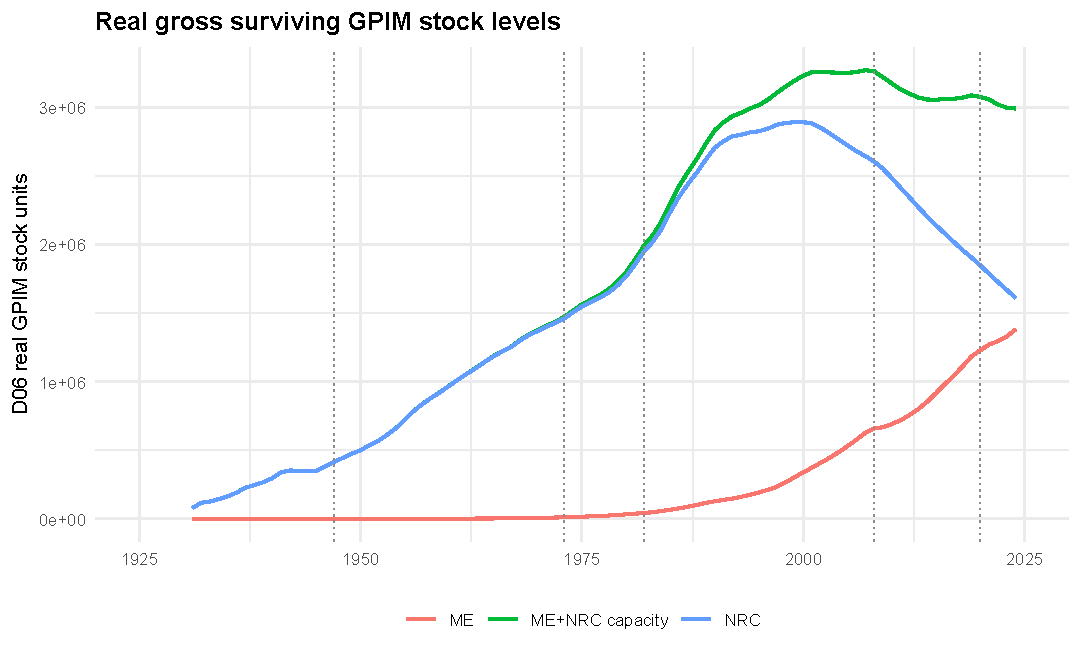
\includegraphics[width=0.92\linewidth]{../figures/D09_fig01_real_gpim_stock_levels.pdf}
\caption{Real gross surviving GPIM stock levels. Baseline D06/D07 refrozen real gross surviving GPIM stocks or report-only visual indices from D09 figure data. The object is source-of-truth only at the underlying level variables; the index view is REPORT\_ONLY and INSPECTION\_ONLY. The NRC path is interpreted as a nonfinancial productive-capacity boundary object, not a literal census of every standing building.}
\label{fig:D09_fig01_real_gpim_stock_levels}
\end{figure}

\begin{figure}[H]
\centering
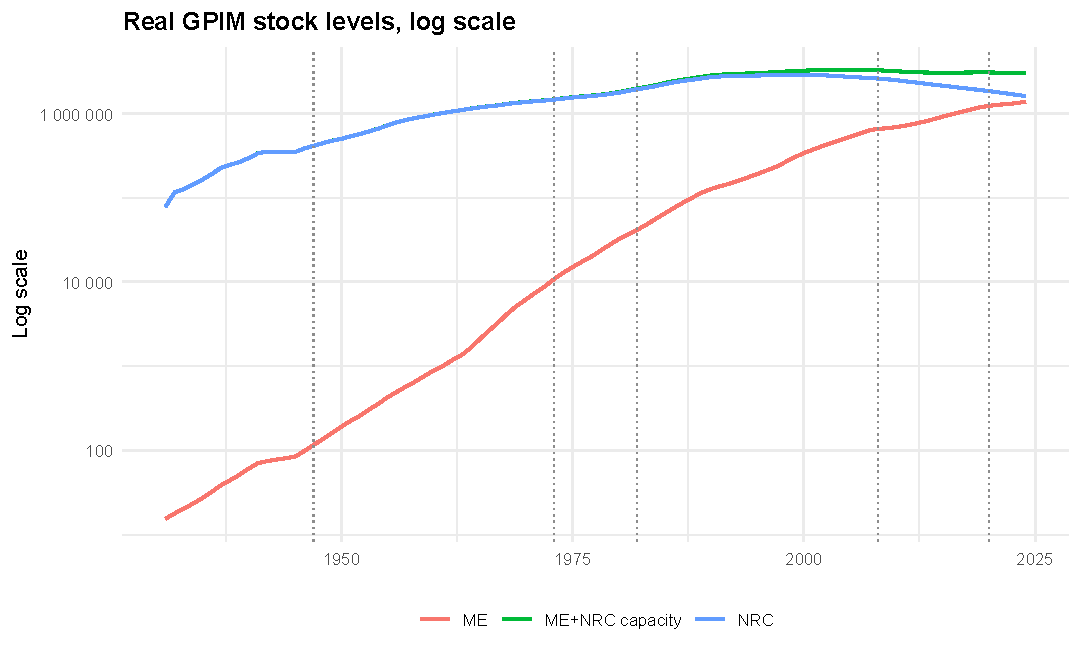
\includegraphics[width=0.92\linewidth]{../figures/D09_fig03_real_gpim_stock_levels_logscale.pdf}
\caption{Real gross surviving GPIM stock levels, log scale. Baseline D06/D07 refrozen real gross surviving GPIM stocks or report-only visual indices from D09 figure data. The object is source-of-truth only at the underlying level variables; the index view is REPORT\_ONLY and INSPECTION\_ONLY. The NRC path is interpreted as a nonfinancial productive-capacity boundary object, not a literal census of every standing building.}
\label{fig:D09_fig03_real_gpim_stock_levels_logscale}
\end{figure}

\begin{figure}[H]
\centering
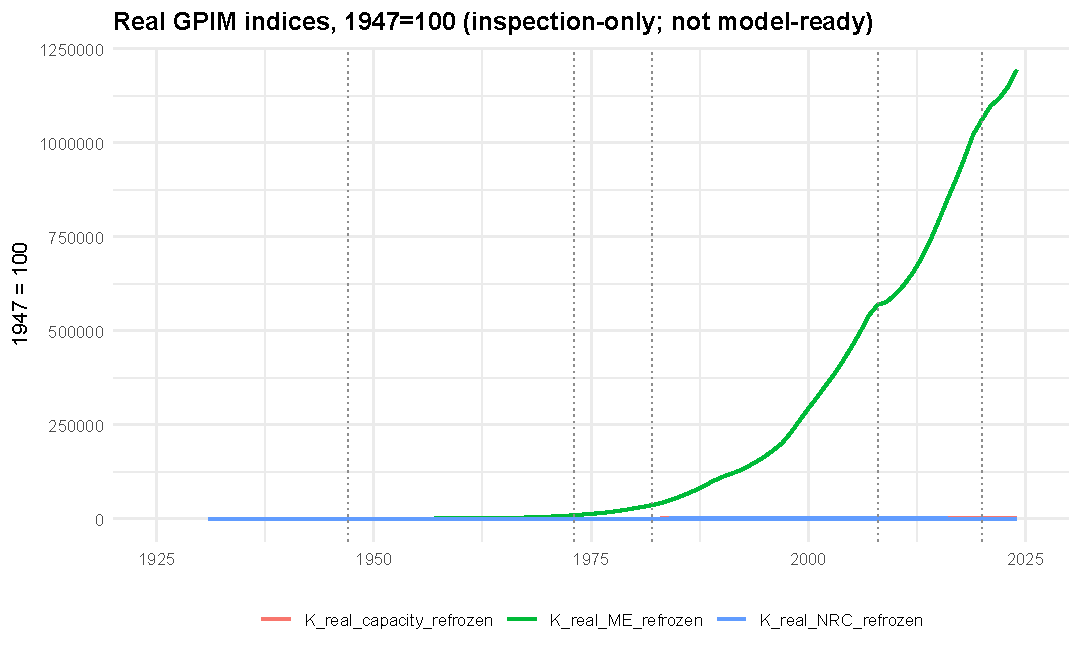
\includegraphics[width=0.92\linewidth]{../figures/D09_fig05_real_gpim_indices_1947_100.pdf}
\caption{Real GPIM visual indices, 1947=100. Baseline D06/D07 refrozen real gross surviving GPIM stocks or report-only visual indices from D09 figure data. The object is source-of-truth only at the underlying level variables; the index view is REPORT\_ONLY and INSPECTION\_ONLY. The NRC path is interpreted as a nonfinancial productive-capacity boundary object, not a literal census of every standing building.}
\label{fig:D09_fig05_real_gpim_indices_1947_100}
\end{figure}

\begin{figure}[H]
\centering
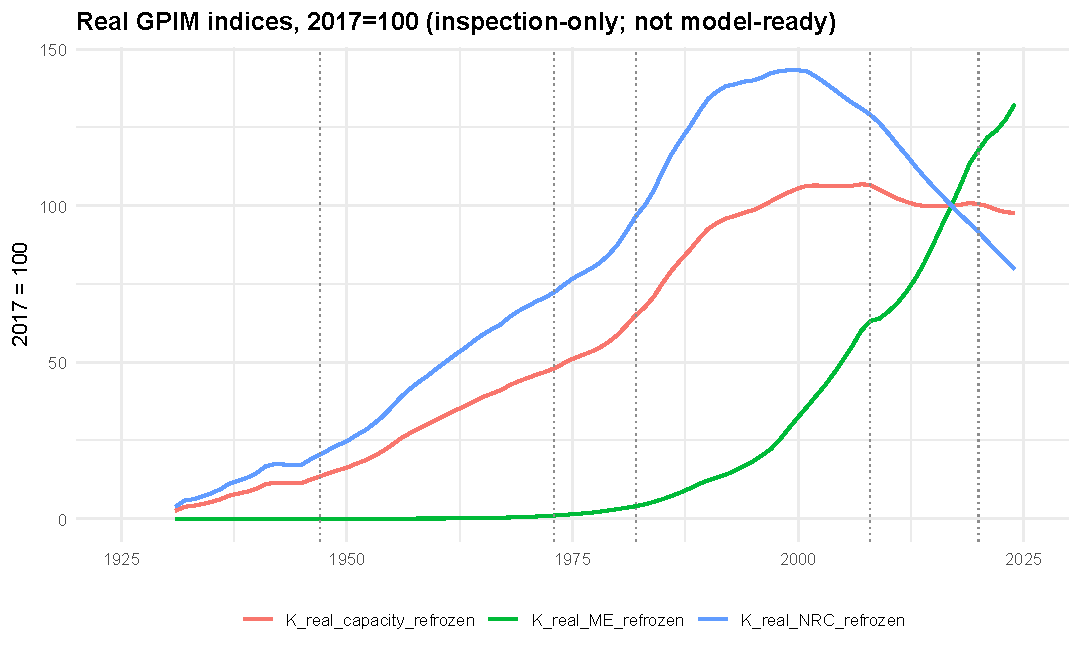
\includegraphics[width=0.92\linewidth]{../figures/D09_fig06_real_gpim_indices_2017_100.pdf}
\caption{Real GPIM visual indices, 2017=100. Baseline D06/D07 refrozen real gross surviving GPIM stocks or report-only visual indices from D09 figure data. The object is source-of-truth only at the underlying level variables; the index view is REPORT\_ONLY and INSPECTION\_ONLY. The NRC path is interpreted as a nonfinancial productive-capacity boundary object, not a literal census of every standing building.}
\label{fig:D09_fig06_real_gpim_indices_2017_100}
\end{figure}

\FloatBarrier
\section{GPIM Current-Cost Stock Levels and Valuation Interpretation}
This section separates current-cost stocks from real stocks. Figures \textbackslash\{\}ref\{fig:D09\_fig02\_current\_cost\_gpim\_stock\_levels\}, \textbackslash\{\}ref\{fig:D09\_fig04\_current\_cost\_gpim\_stock\_levels\_logscale\}, \textbackslash\{\}ref\{fig:D09\_fig07\_current\_cost\_gpim\_indices\_1947\_100\}, \textbackslash\{\}ref\{fig:D09\_fig08\_current\_cost\_gpim\_indices\_2017\_100\} show levels and report-only indices after pKN valuation enters the accounting object.

Current-cost paths mix quantity and valuation effects. A current-cost increase can coexist with real-stock stagnation or decline if pKN movements offset real quantity movements; the interpretation therefore cannot be read as a pure physical-capacity path.

This section does not change pKN and does not use current-cost paths as a substitute for real-capacity validation.
\begin{figure}[H]
\centering
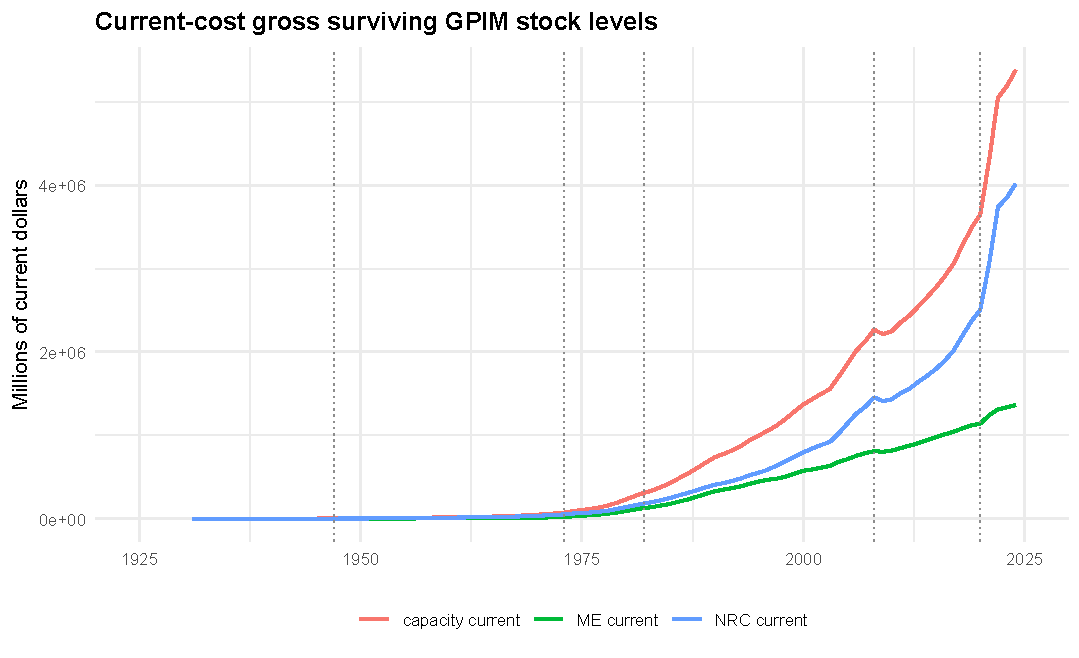
\includegraphics[width=0.92\linewidth]{../figures/D09_fig02_current_cost_gpim_stock_levels.pdf}
\caption{Current-cost gross surviving GPIM stock levels. Baseline D06/D07 current-cost GPIM levels or D09 report-only current-cost visual indices. These paths mix quantity and valuation effects through pKN support and are not model transformations.}
\label{fig:D09_fig02_current_cost_gpim_stock_levels}
\end{figure}

\begin{figure}[H]
\centering
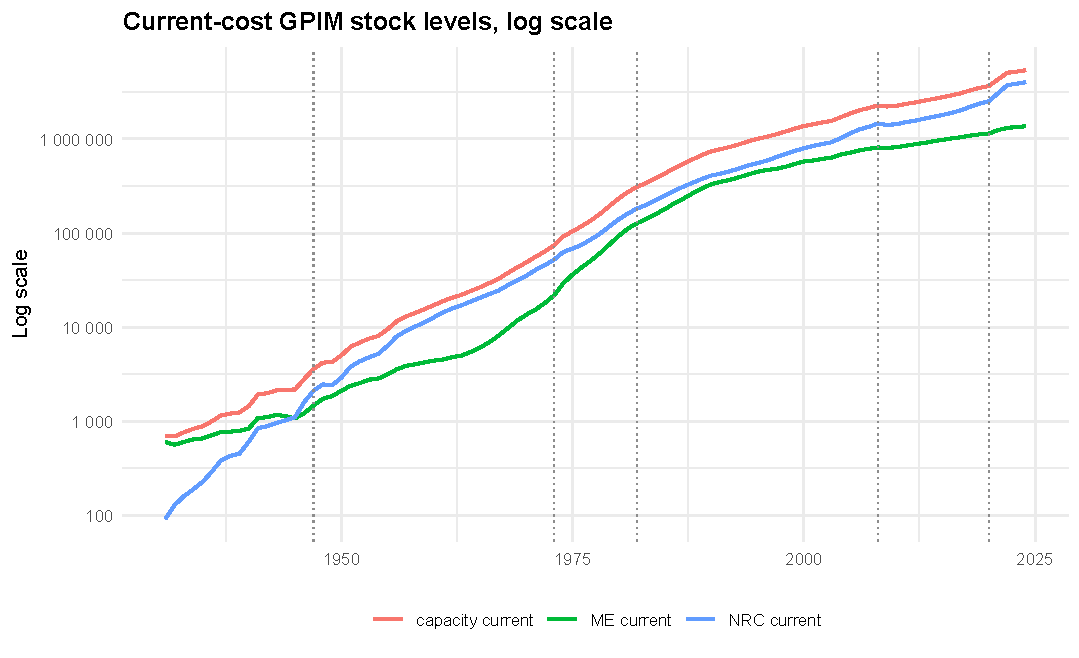
\includegraphics[width=0.92\linewidth]{../figures/D09_fig04_current_cost_gpim_stock_levels_logscale.pdf}
\caption{Current-cost gross surviving GPIM stock levels, log scale. Baseline D06/D07 current-cost GPIM levels or D09 report-only current-cost visual indices. These paths mix quantity and valuation effects through pKN support and are not model transformations.}
\label{fig:D09_fig04_current_cost_gpim_stock_levels_logscale}
\end{figure}

\begin{figure}[H]
\centering
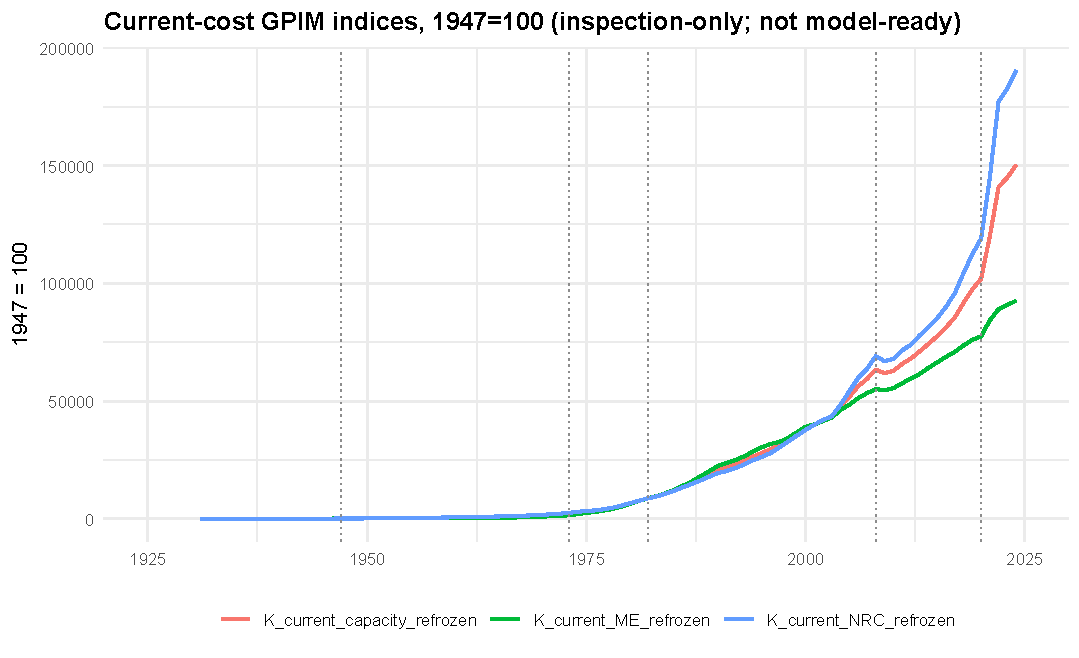
\includegraphics[width=0.92\linewidth]{../figures/D09_fig07_current_cost_gpim_indices_1947_100.pdf}
\caption{Current-cost GPIM visual indices, 1947=100. Baseline D06/D07 current-cost GPIM levels or D09 report-only current-cost visual indices. These paths mix quantity and valuation effects through pKN support and are not model transformations.}
\label{fig:D09_fig07_current_cost_gpim_indices_1947_100}
\end{figure}

\begin{figure}[H]
\centering
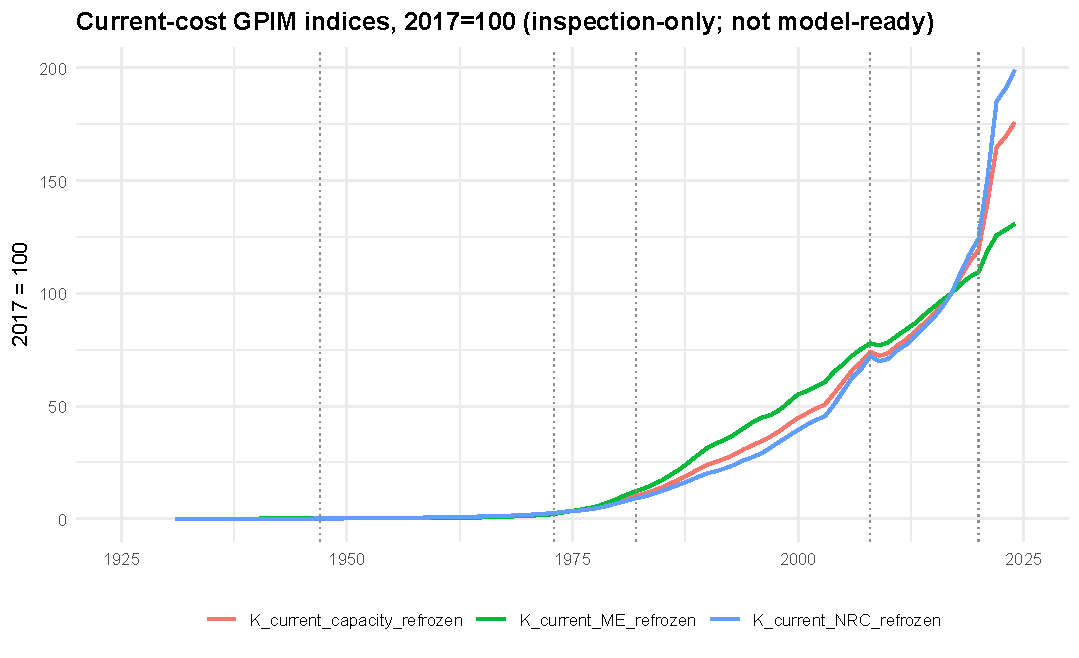
\includegraphics[width=0.92\linewidth]{../figures/D09_fig08_current_cost_gpim_indices_2017_100.pdf}
\caption{Current-cost GPIM visual indices, 2017=100. Baseline D06/D07 current-cost GPIM levels or D09 report-only current-cost visual indices. These paths mix quantity and valuation effects through pKN support and are not model transformations.}
\label{fig:D09_fig08_current_cost_gpim_indices_2017_100}
\end{figure}

\FloatBarrier
\section{Warmup, Survival Profiles, and the NRC Service-Life Concern}
This section places warmup and survival directly before the identity checks because the NRC concern is a service-life and initialization concern. Figures \textbackslash\{\}ref\{fig:D09\_fig09\_gpim\_warmup\_timeline\}, \textbackslash\{\}ref\{fig:D09\_fig10\_locked\_survival\_profiles\_ME\_NRC\} show the warmup timeline and locked survival profiles.

ME warmup is likely adequate relative to L=14. NRC warmup is review-required relative to L=30. The review flag is non-blocking in D08/D09 because identities, pKN normalization, real-investment scale, current-cost valuation, and source-consumption checks pass.

This section does not change L=30 or alpha=1.6 for NRC. It records the concern and points to future sensitivity design.
\begin{figure}[H]
\centering
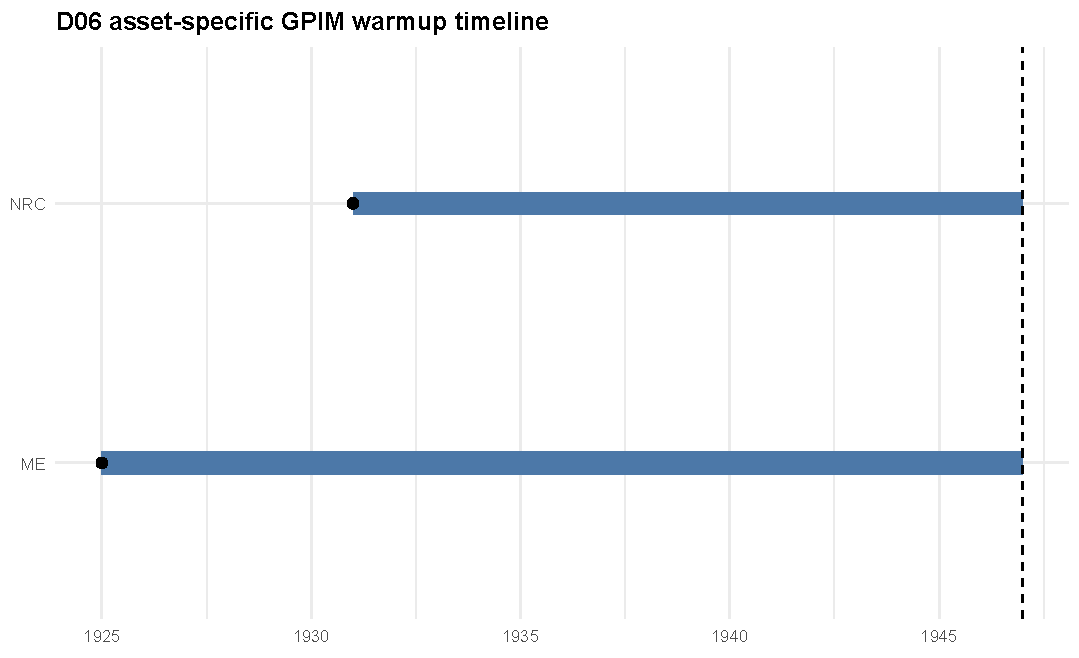
\includegraphics[width=0.92\linewidth]{../figures/D09_fig09_gpim_warmup_timeline.pdf}
\caption{Asset-specific GPIM warmup timeline. D08/D09 diagnostic figure using locked D06 survival parameters. ME L=14 is likely adequate after warmup; NRC L=30 remains REVIEW\_REQUIRED. D09-R does not change L, alpha, warmup, or GPIM stocks.}
\label{fig:D09_fig09_gpim_warmup_timeline}
\end{figure}

\begin{figure}[H]
\centering
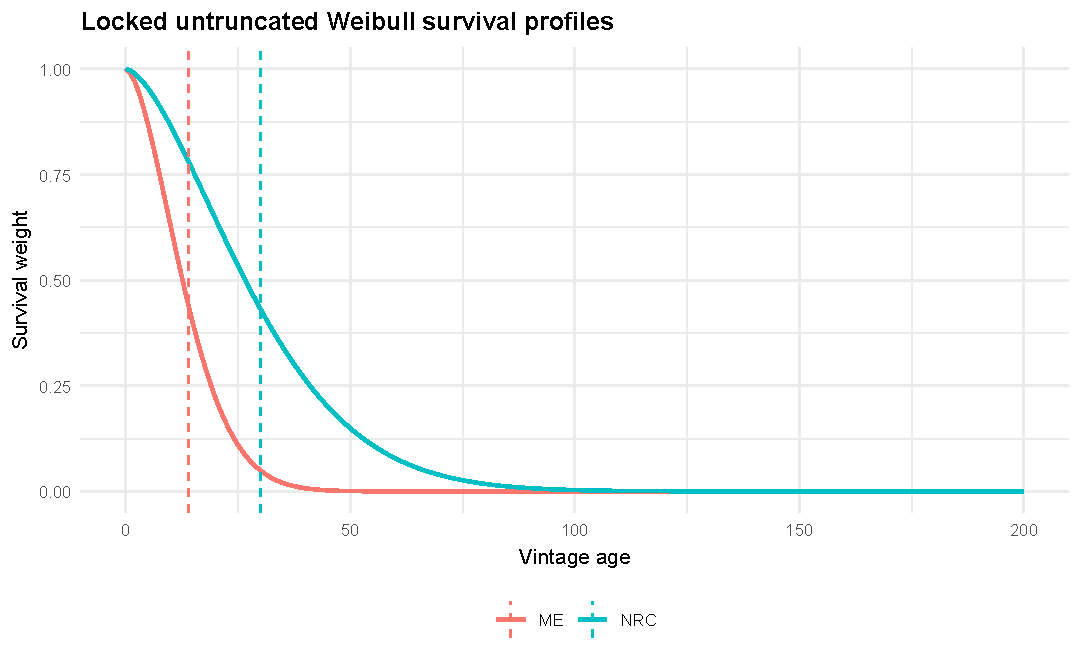
\includegraphics[width=0.92\linewidth]{../figures/D09_fig10_locked_survival_profiles_ME_NRC.pdf}
\caption{Locked untruncated Weibull survival profiles. D08/D09 diagnostic figure using locked D06 survival parameters. ME L=14 is likely adequate after warmup; NRC L=30 remains REVIEW\_REQUIRED. D09-R does not change L, alpha, warmup, or GPIM stocks.}
\label{fig:D09_fig10_locked_survival_profiles_ME_NRC}
\end{figure}

\input{../tables/D09_R_table_warmup_sufficiency.tex}

\begin{tabular}{lllll}
\toprule
issue\_id & risk\_level & blocking\_status & interpretation & recommended\_followup\\
\midrule
NRC\_REAL\_GROSS\_STOCK\_DECLINE & MEDIUM & REVIEW\_REQUIRED & The decline or stagnation is a productive-capacity boundary movement, not literal demolition of every structure. & Review figures and carry NRC service-life concern into future sensitivity.\\
NRC\_WARMUP\_SHORT\_RELATIVE\_TO\_L30 & MEDIUM & REVIEW\_REQUIRED & Warmup is non-blocking because D08/D09 identity, scale, pKN, and consumption checks pass. & Design sensitivity cases for longer NRC service lives and warmup treatment.\\
NRC\_L30\_SERVICE\_LIFE\_UNCERTAINTY & MEDIUM & REVIEW\_REQUIRED & The L=30 assumption can shape the real NRC trajectory and should be tested later. & Retrieve and verify service-life literature before choosing alternatives.\\
SECTOR\_BOUNDARY\_NONFINANCIAL\_STRUCTURES & MEDIUM & REVIEW\_REQUIRED & The object can be defended only as nonfinancial productive-capacity NRC, not as all nonresidential structures. & Maintain ME+NRC boundary; do not add parked assets.\\
PHYSICAL\_BUILDING\_STOCK\_VS\_PRODUCTIVE\_CAPACITY\_STOCK & MEDIUM & REVIEW\_REQUIRED & A building can stand while exiting the analytical productive-capacity boundary. & Keep captions explicit about productive-capacity scope.\\
\addlinespace
REZONING\_CONVERSION\_ABANDONMENT\_INTERPRETATION & MEDIUM & REVIEW\_REQUIRED & Rezoning, conversion to residential use, and abandonment are plausible boundary mechanisms. & Document possible boundary exits without quantifying them in D09-R.\\
FINANCIAL\_NONPRODUCTIVE\_ABSORPTION\_INTERPRETATION & MEDIUM & REVIEW\_REQUIRED & Financial or real-estate absorption can remove a structure from the productive-capacity interpretation. & Keep financial correction as transfer/reconciliation layer.\\
FUTURE\_SENSITIVITY\_NEED & MEDIUM & REVIEW\_REQUIRED & D09-R authorizes only double validation review, not D10 transformation planning. & Run a future report-only sensitivity appendix or D10 precheck.\\
\bottomrule
\end{tabular}

\FloatBarrier
\section{Stock-Flow and Current-Cost Identity Audits}
This section comes before composition and ratio plots because accounting coherence must be visible before derived diagnostics. Figures \textbackslash\{\}ref\{fig:D09\_fig11\_real\_investment\_scale\_residuals\}, \textbackslash\{\}ref\{fig:D09\_fig12\_current\_cost\_identity\_residuals\}, \textbackslash\{\}ref\{fig:D09\_fig13\_capacity\_identity\_residuals\} display the real-investment scale, current-cost valuation, and capacity aggregation residuals.

The residual evidence supports the D08 conclusion that the GPIM repair did not break the required identities. This is why the NRC service-life issue remains review-required rather than blocking at D09-R.

These plots are audits, not regressions or transformation diagnostics. They do not authorize D10 use.
\begin{figure}[H]
\centering
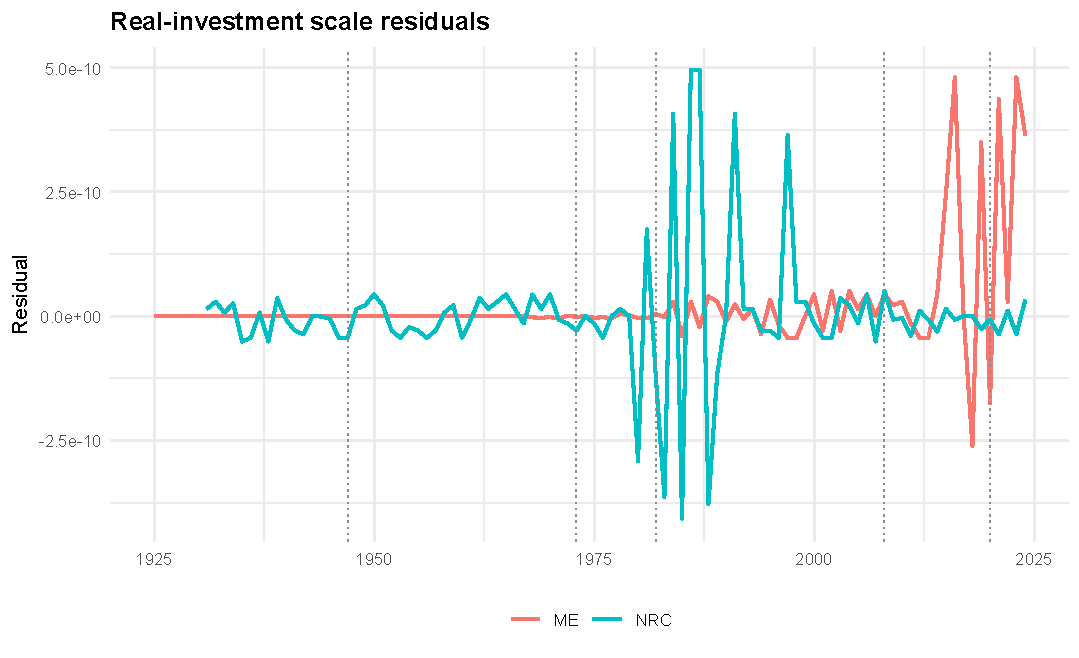
\includegraphics[width=0.92\linewidth]{../figures/D09_fig11_real_investment_scale_residuals.pdf}
\caption{Real-investment scale residuals. D08/D09 audit diagnostic showing identity or scale residuals. The plotted object is an accounting validation diagnostic, not an econometric result and not a new source-of-truth variable.}
\label{fig:D09_fig11_real_investment_scale_residuals}
\end{figure}

\begin{figure}[H]
\centering
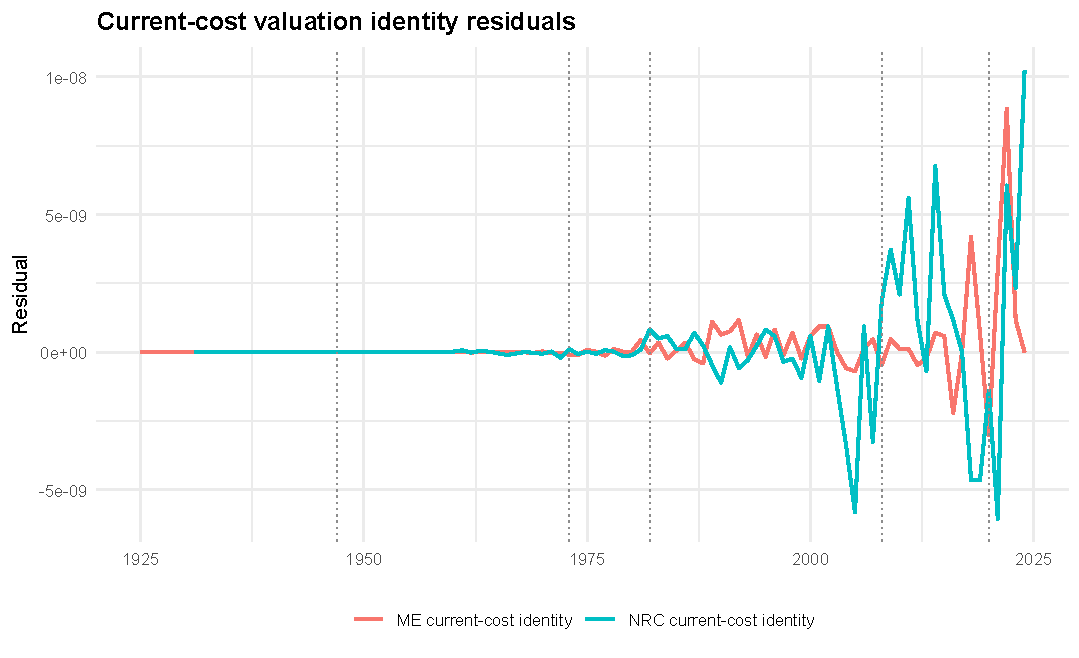
\includegraphics[width=0.92\linewidth]{../figures/D09_fig12_current_cost_identity_residuals.pdf}
\caption{Current-cost valuation identity residuals. D08/D09 audit diagnostic showing identity or scale residuals. The plotted object is an accounting validation diagnostic, not an econometric result and not a new source-of-truth variable.}
\label{fig:D09_fig12_current_cost_identity_residuals}
\end{figure}

\begin{figure}[H]
\centering
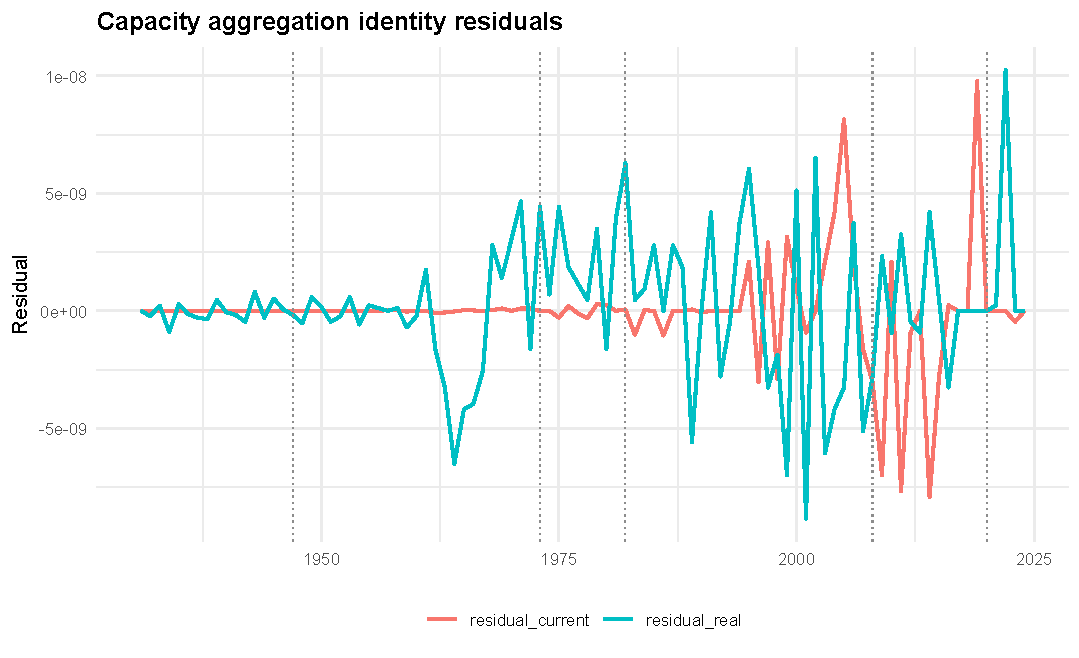
\includegraphics[width=0.92\linewidth]{../figures/D09_fig13_capacity_identity_residuals.pdf}
\caption{Capacity aggregation identity residuals. D08/D09 audit diagnostic showing identity or scale residuals. The plotted object is an accounting validation diagnostic, not an econometric result and not a new source-of-truth variable.}
\label{fig:D09_fig13_capacity_identity_residuals}
\end{figure}

\input{../tables/D09_R_table_gpim_identity_residuals.tex}
\FloatBarrier
\section{ME/NRC Composition and Mechanization Diagnostics}
This section groups the ME/NRC ratios and shares so the reader can see composition after the level and identity evidence. Figures \textbackslash\{\}ref\{fig:D09\_fig14\_ME\_over\_NRC\_real\_stock\_ratio\}, \textbackslash\{\}ref\{fig:D09\_fig15\_ME\_over\_NRC\_current\_stock\_ratio\}, \textbackslash\{\}ref\{fig:D09\_fig16\_ME\_NRC\_real\_capacity\_shares\}, \textbackslash\{\}ref\{fig:D09\_fig17\_ME\_NRC\_current\_capacity\_shares\}, \textbackslash\{\}ref\{fig:D09\_fig18\_ME\_over\_NRC\_real\_investment\_ratio\}, \textbackslash\{\}ref\{fig:D09\_fig19\_ME\_over\_NRC\_current\_investment\_ratio\} compare real, current-cost, and investment composition.

The composition figures make the mechanization and construction mix visible without creating a new source variable. They are useful precisely because they are downstream inspection objects with the baseline ME/NRC boundary intact.

No composition ratio is model-ready in D09-R. Any use as q or another transformation requires later D10 authorization.
\begin{figure}[H]
\centering
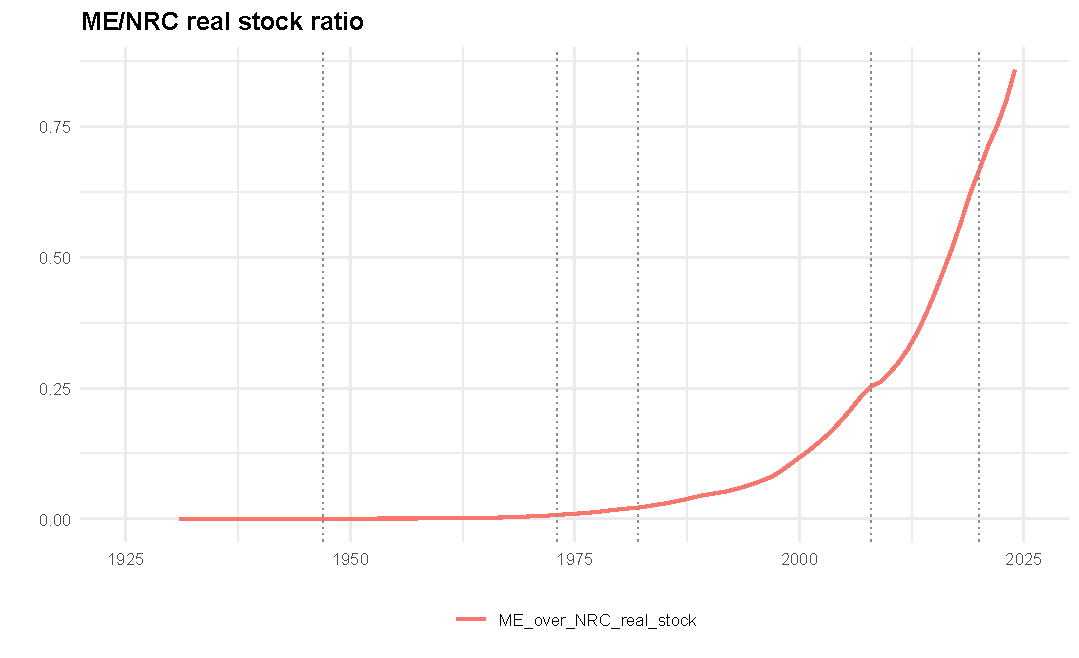
\includegraphics[width=0.92\linewidth]{../figures/D09_fig14_ME_over_NRC_real_stock_ratio.pdf}
\caption{ME/NRC real stock ratio. Report-only ME/NRC composition diagnostic from D09 figure data. It compares D06/D07 baseline ME and NRC components inside the nonfinancial capacity-capital boundary and is not a model transformation unless D10 later authorizes it.}
\label{fig:D09_fig14_ME_over_NRC_real_stock_ratio}
\end{figure}

\begin{figure}[H]
\centering
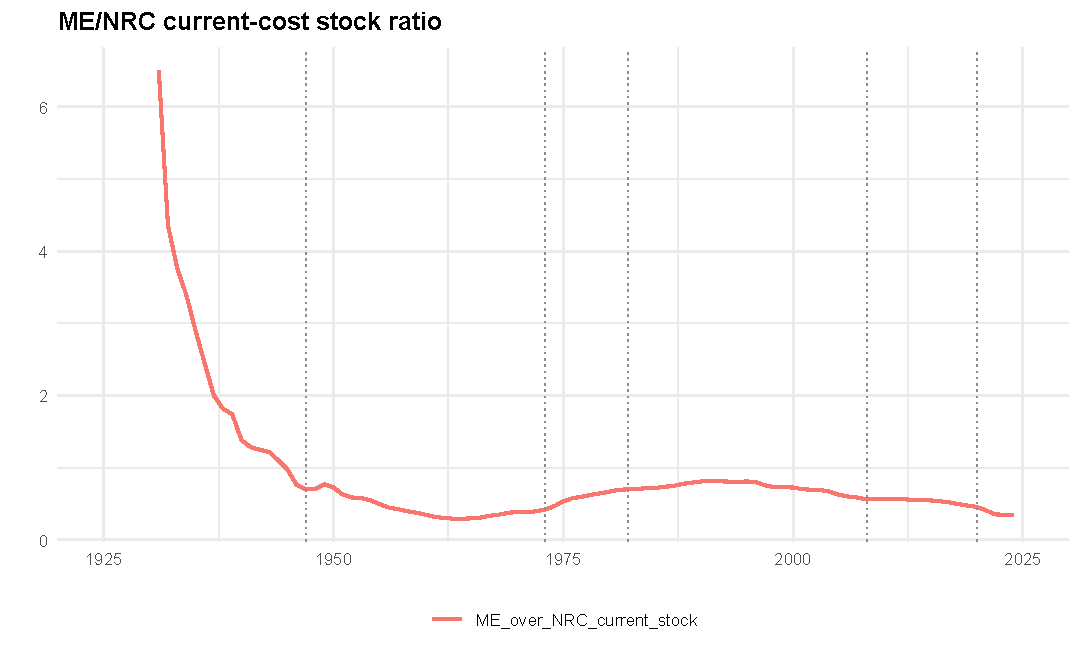
\includegraphics[width=0.92\linewidth]{../figures/D09_fig15_ME_over_NRC_current_stock_ratio.pdf}
\caption{ME/NRC current-cost stock ratio. Report-only ME/NRC composition diagnostic from D09 figure data. It compares D06/D07 baseline ME and NRC components inside the nonfinancial capacity-capital boundary and is not a model transformation unless D10 later authorizes it.}
\label{fig:D09_fig15_ME_over_NRC_current_stock_ratio}
\end{figure}

\begin{figure}[H]
\centering
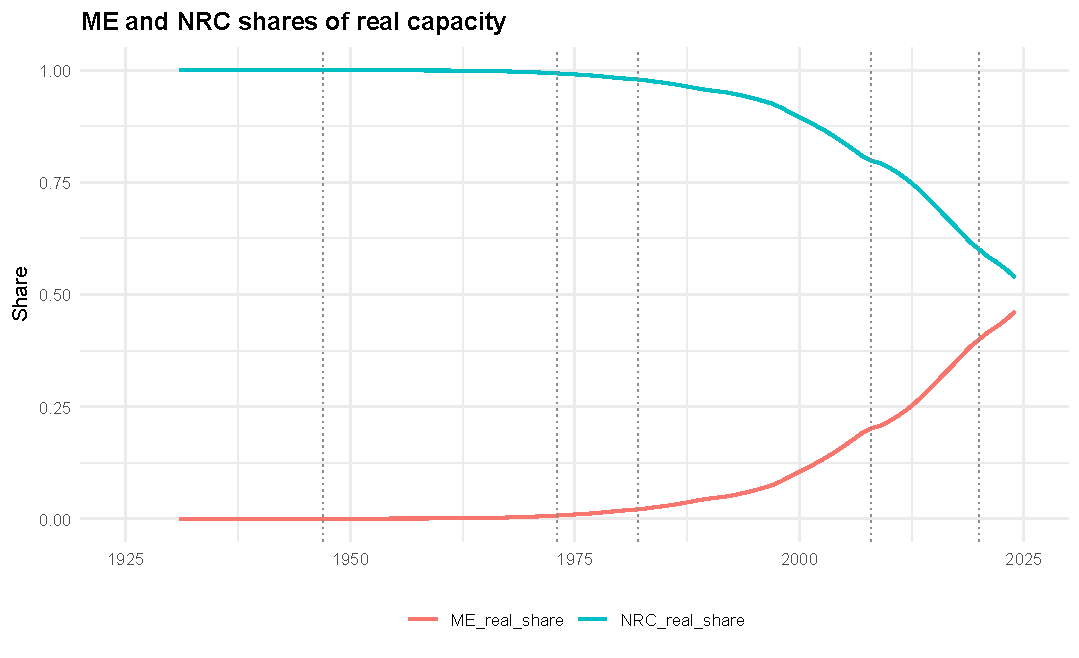
\includegraphics[width=0.92\linewidth]{../figures/D09_fig16_ME_NRC_real_capacity_shares.pdf}
\caption{ME and NRC shares of real capacity. Report-only ME/NRC composition diagnostic from D09 figure data. It compares D06/D07 baseline ME and NRC components inside the nonfinancial capacity-capital boundary and is not a model transformation unless D10 later authorizes it.}
\label{fig:D09_fig16_ME_NRC_real_capacity_shares}
\end{figure}

\begin{figure}[H]
\centering
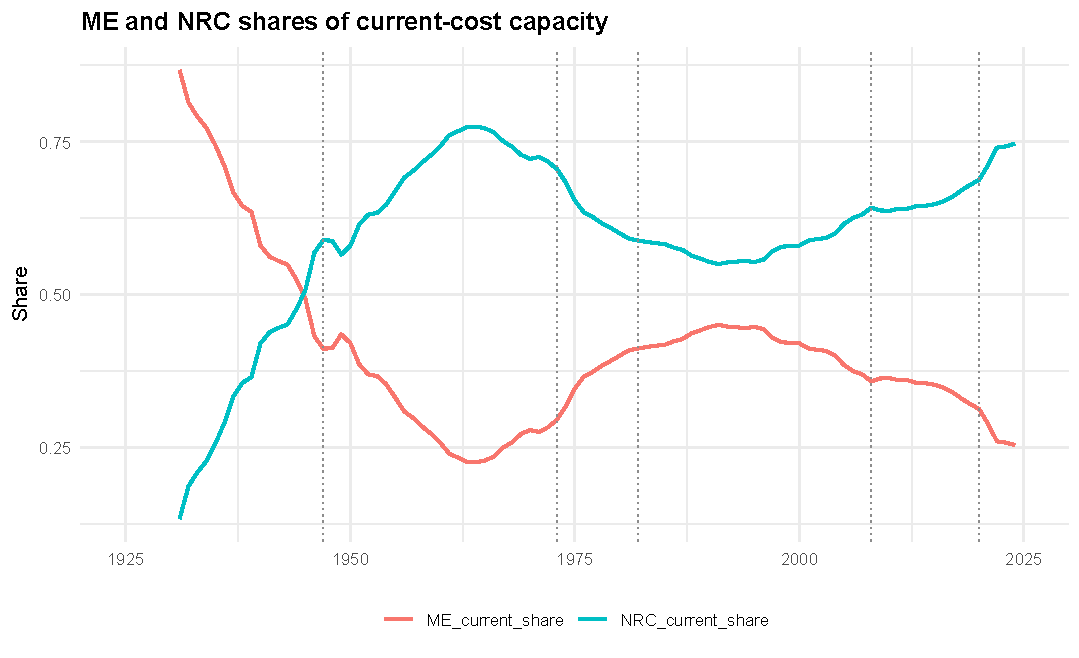
\includegraphics[width=0.92\linewidth]{../figures/D09_fig17_ME_NRC_current_capacity_shares.pdf}
\caption{ME and NRC shares of current-cost capacity. Report-only ME/NRC composition diagnostic from D09 figure data. It compares D06/D07 baseline ME and NRC components inside the nonfinancial capacity-capital boundary and is not a model transformation unless D10 later authorizes it.}
\label{fig:D09_fig17_ME_NRC_current_capacity_shares}
\end{figure}

\begin{figure}[H]
\centering
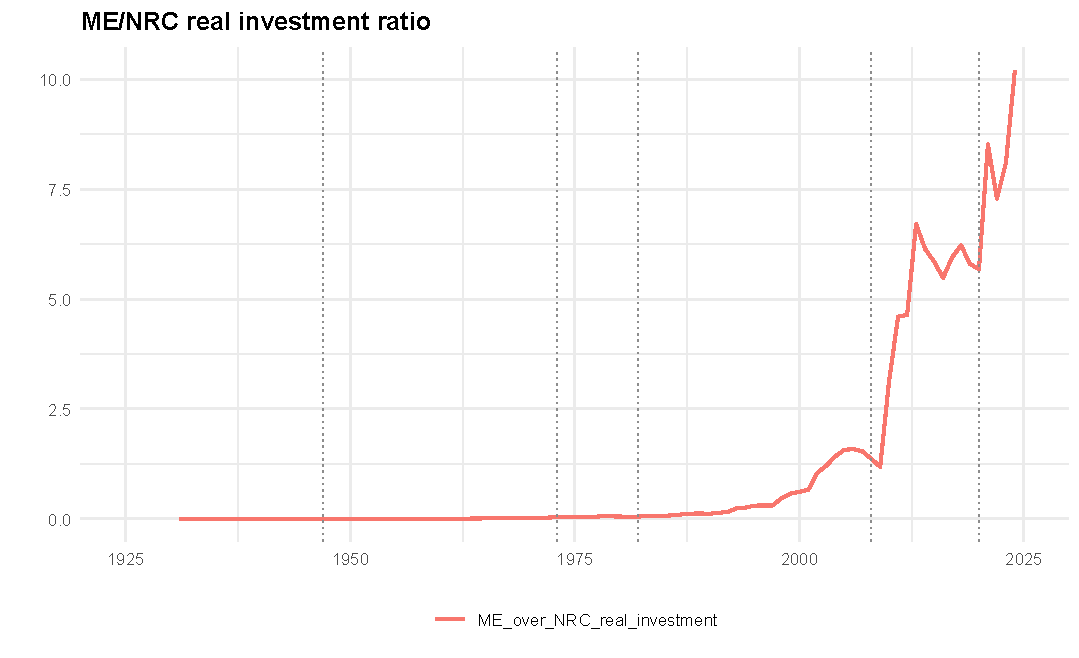
\includegraphics[width=0.92\linewidth]{../figures/D09_fig18_ME_over_NRC_real_investment_ratio.pdf}
\caption{ME/NRC real investment ratio. Report-only ME/NRC composition diagnostic from D09 figure data. It compares D06/D07 baseline ME and NRC components inside the nonfinancial capacity-capital boundary and is not a model transformation unless D10 later authorizes it.}
\label{fig:D09_fig18_ME_over_NRC_real_investment_ratio}
\end{figure}

\begin{figure}[H]
\centering
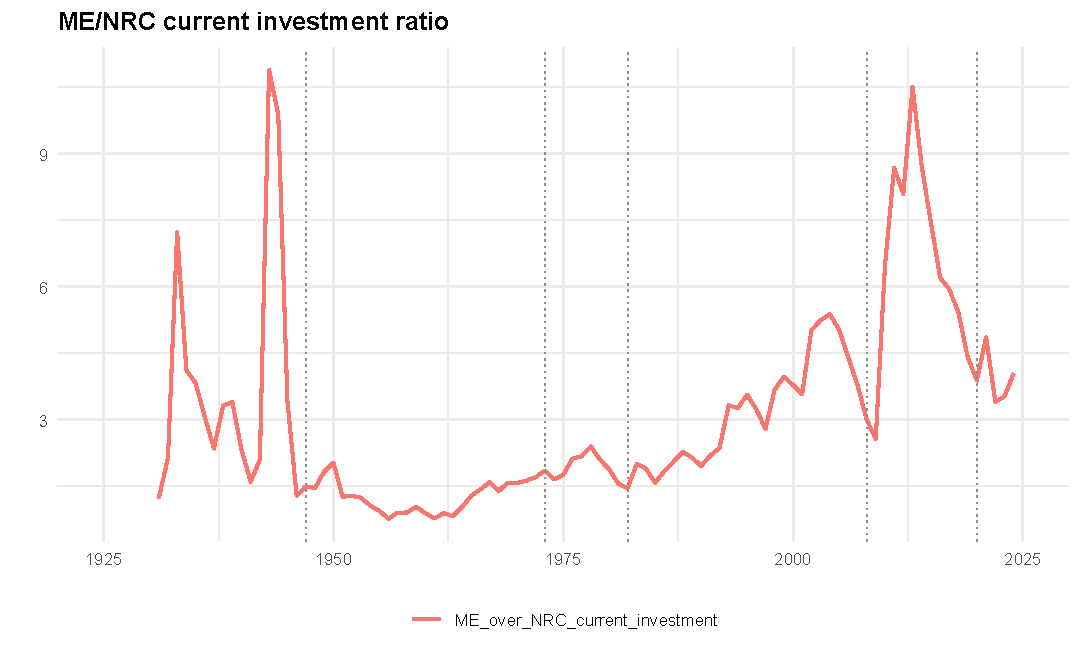
\includegraphics[width=0.92\linewidth]{../figures/D09_fig19_ME_over_NRC_current_investment_ratio.pdf}
\caption{ME/NRC current investment ratio. Report-only ME/NRC composition diagnostic from D09 figure data. It compares D06/D07 baseline ME and NRC components inside the nonfinancial capacity-capital boundary and is not a model transformation unless D10 later authorizes it.}
\label{fig:D09_fig19_ME_over_NRC_current_investment_ratio}
\end{figure}

\FloatBarrier
\section{Net-over-Gross Comparisons and Concept Boundaries}
This section isolates net-over-gross diagnostics from baseline capital measures. Figures \textbackslash\{\}ref\{fig:D09\_fig20\_net\_over\_gross\_current\_cost\_ME\}, \textbackslash\{\}ref\{fig:D09\_fig21\_net\_over\_gross\_current\_cost\_NRC\}, \textbackslash\{\}ref\{fig:D09\_fig22\_net\_over\_gross\_current\_cost\_capacity\} compare current-cost net-stock concepts with current-cost gross GPIM stocks where those comparisons are available.

Net-over-gross comparisons are accounting diagnostics, not substitutes for the D06 gross surviving GPIM baseline. They compare current-cost net stock concepts to current-cost gross GPIM stocks where available.

The section does not replace the baseline with net stocks and does not promote accounting comparisons to source-of-truth status.
\begin{figure}[H]
\centering
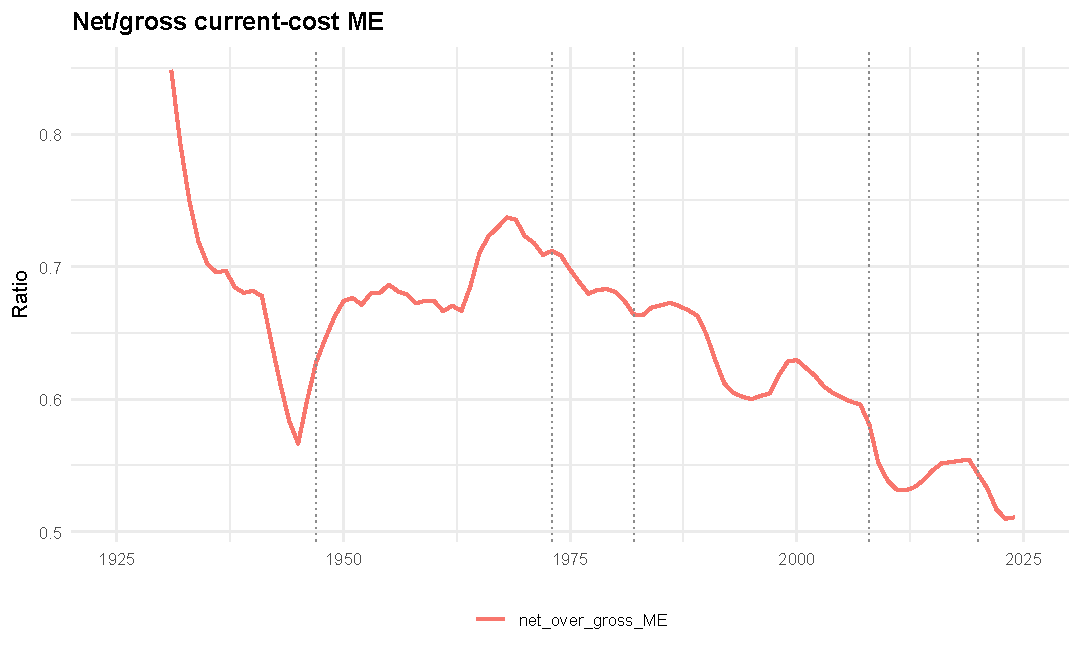
\includegraphics[width=0.92\linewidth]{../figures/D09_fig20_net_over_gross_current_cost_ME.pdf}
\caption{Net/gross current-cost ME. Accounting-comparison diagnostic from D09 figure data. Net-over-gross comparisons are not substitutes for the D06 gross surviving GPIM baseline; they compare current-cost net stock concepts to current-cost gross GPIM stocks where available.}
\label{fig:D09_fig20_net_over_gross_current_cost_ME}
\end{figure}

\begin{figure}[H]
\centering
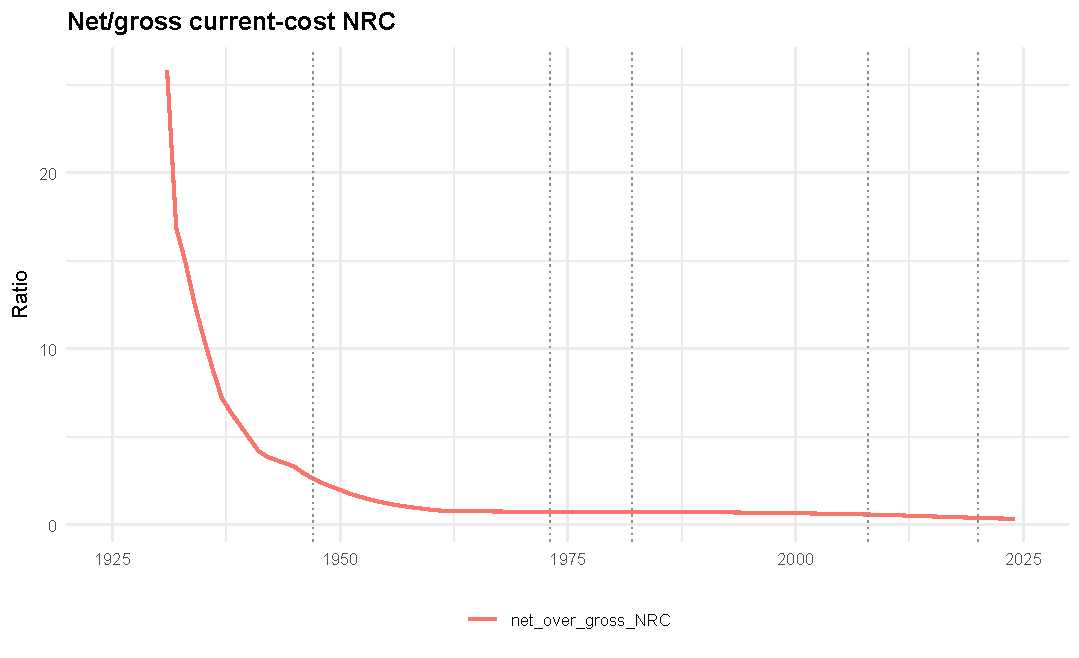
\includegraphics[width=0.92\linewidth]{../figures/D09_fig21_net_over_gross_current_cost_NRC.pdf}
\caption{Net/gross current-cost NRC. Accounting-comparison diagnostic from D09 figure data. Net-over-gross comparisons are not substitutes for the D06 gross surviving GPIM baseline; they compare current-cost net stock concepts to current-cost gross GPIM stocks where available.}
\label{fig:D09_fig21_net_over_gross_current_cost_NRC}
\end{figure}

\begin{figure}[H]
\centering
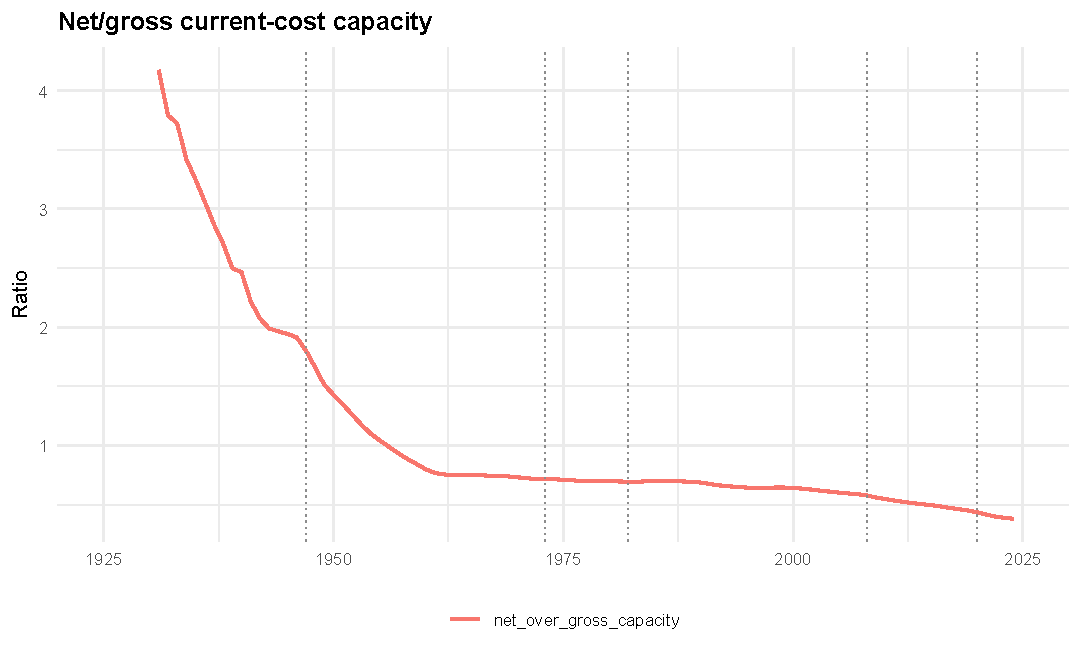
\includegraphics[width=0.92\linewidth]{../figures/D09_fig22_net_over_gross_current_cost_capacity.pdf}
\caption{Net/gross current-cost capacity. Accounting-comparison diagnostic from D09 figure data. Net-over-gross comparisons are not substitutes for the D06 gross surviving GPIM baseline; they compare current-cost net stock concepts to current-cost gross GPIM stocks where available.}
\label{fig:D09_fig22_net_over_gross_current_cost_capacity}
\end{figure}

\FloatBarrier
\section{Capital-Measure Status Map: Baseline, Comparison, Review-Only, Parked, Excluded}
This section repairs the status-map flow by placing the status map, baseline comparison, and parked/excluded view together. Figures \textbackslash\{\}ref\{fig:D09\_fig23\_capital\_measure\_status\_map\}, \textbackslash\{\}ref\{fig:D09\_fig24\_baseline\_vs\_accounting\_comparison\_capital\}, \textbackslash\{\}ref\{fig:D09\_fig25\_parked\_excluded\_capital\_objects\_appendix\} show which capital objects are baseline, comparison, review-only, parked, or excluded.

The parked/excluded figure is kept in the main status section only as a boundary-warning device. It prevents the reader from mistaking broader fixed-asset objects for the baseline ME+NRC capacity object.

Parked and excluded objects are not visually promoted as alternatives to baseline. They remain outside transformation use.
\begin{figure}[H]
\centering
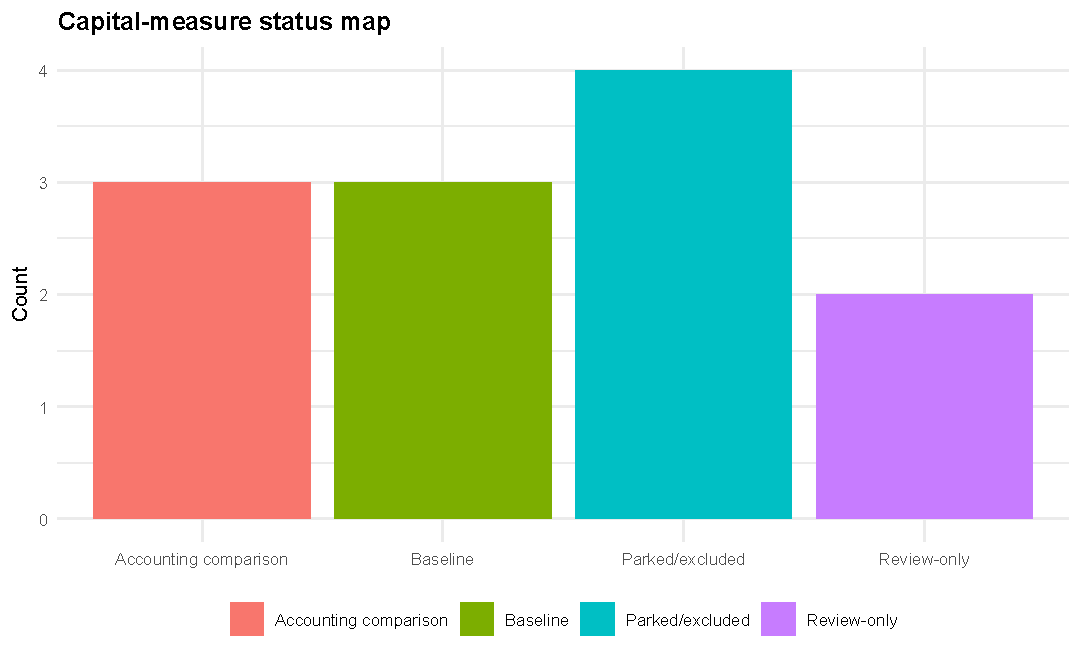
\includegraphics[width=0.92\linewidth]{../figures/D09_fig23_capital_measure_status_map.pdf}
\caption{Capital-measure status map. Boundary-status diagnostic separating baseline, accounting-comparison, review-only, parked, and excluded objects. Parked/excluded objects are shown only to prevent boundary leakage and are not promoted as baseline alternatives.}
\label{fig:D09_fig23_capital_measure_status_map}
\end{figure}

\begin{figure}[H]
\centering
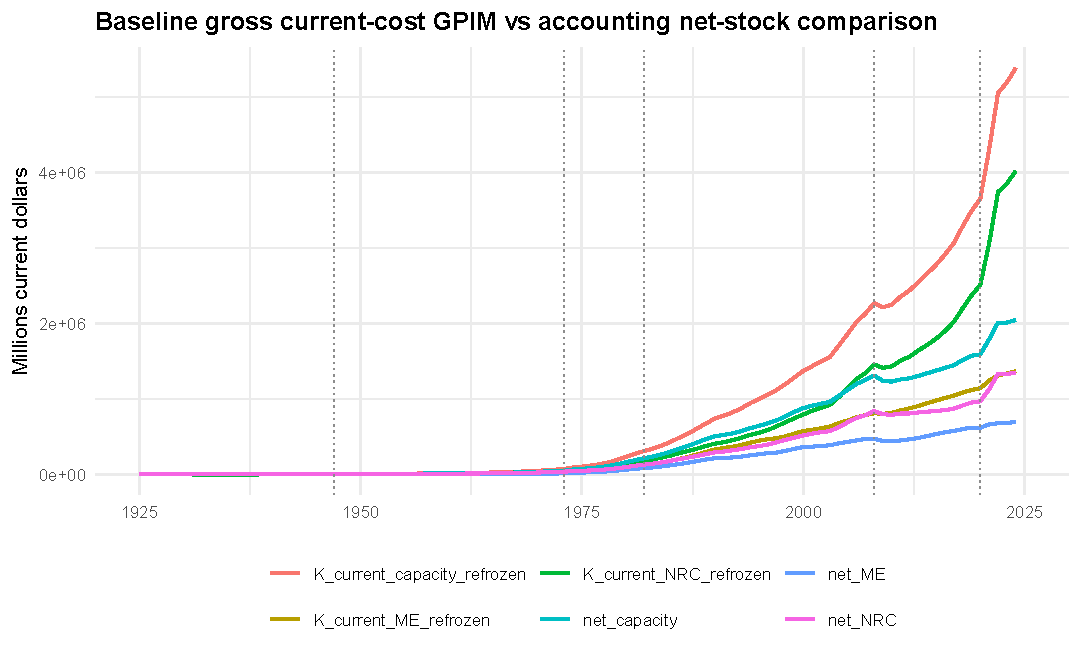
\includegraphics[width=0.92\linewidth]{../figures/D09_fig24_baseline_vs_accounting_comparison_capital.pdf}
\caption{Baseline gross GPIM versus accounting net-stock comparison. Boundary-status diagnostic separating baseline, accounting-comparison, review-only, parked, and excluded objects. Parked/excluded objects are shown only to prevent boundary leakage and are not promoted as baseline alternatives.}
\label{fig:D09_fig24_baseline_vs_accounting_comparison_capital}
\end{figure}

\begin{figure}[H]
\centering
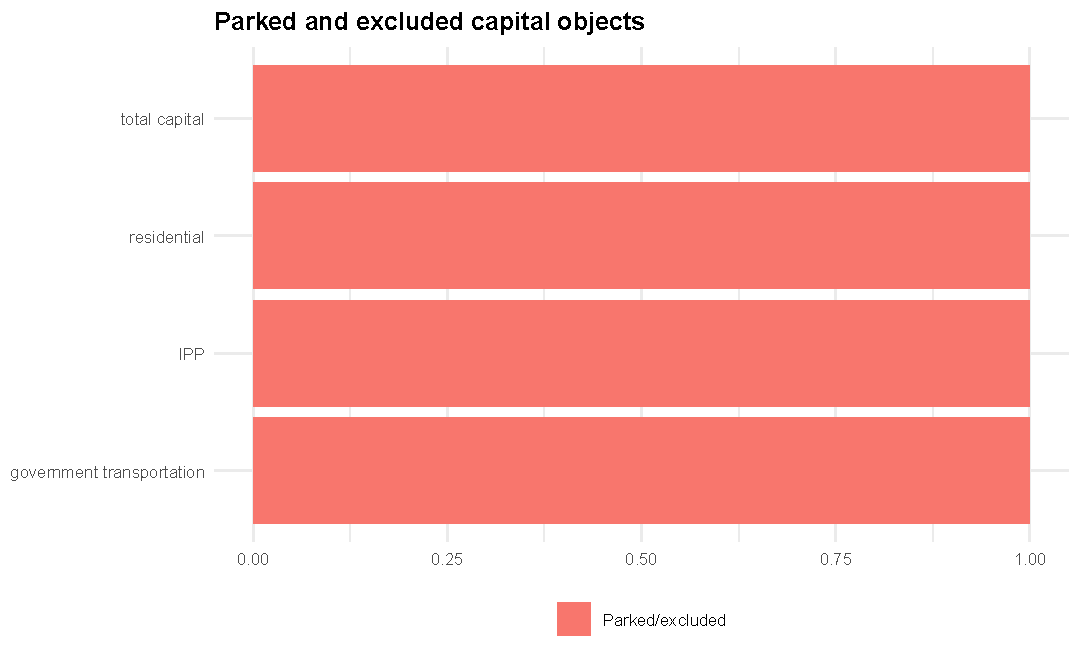
\includegraphics[width=0.92\linewidth]{../figures/D09_fig25_parked_excluded_capital_objects_appendix.pdf}
\caption{Parked and excluded capital objects status view. Boundary-status diagnostic separating baseline, accounting-comparison, review-only, parked, and excluded objects. Parked/excluded objects are shown only to prevent boundary leakage and are not promoted as baseline alternatives.}
\label{fig:D09_fig25_parked_excluded_capital_objects_appendix}
\end{figure}

\FloatBarrier
\section{pKN and Investment-Flow Diagnostics}
This section places pKN and investment diagnostics immediately after the capital-status map because pKN is the bridge between real and current-cost GPIM objects. Figures \textbackslash\{\}ref\{fig:D09\_fig26\_pKN\_ME\_NRC\_capacity\}, \textbackslash\{\}ref\{fig:D09\_fig27\_pKN\_ME\_over\_NRC\}, \textbackslash\{\}ref\{fig:D09\_fig28\_current\_vs\_real\_investment\_ME\}, \textbackslash\{\}ref\{fig:D09\_fig29\_current\_vs\_real\_investment\_NRC\} show price paths, the ME/NRC price ratio, and current-versus-real guarded investment.

pKN movements help explain why current-cost NRC can behave differently from real NRC. They do not by themselves explain away the real NRC path, which remains a real-stock and service-life review question.

D09-R does not alter pKN, does not recalibrate investment, and does not rebuild the real stock.
\begin{figure}[H]
\centering
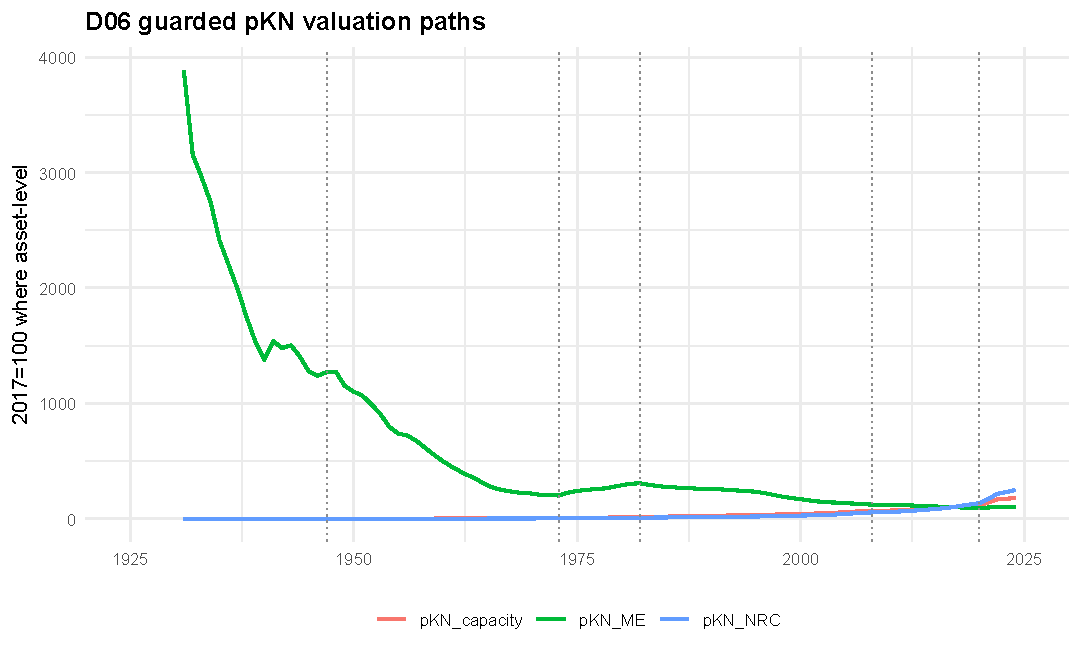
\includegraphics[width=0.92\linewidth]{../figures/D09_fig26_pKN_ME_NRC_capacity.pdf}
\caption{pKN ME, NRC, and capacity paths. D06/D09 pKN and guarded investment-flow diagnostic. The figure helps separate real quantity movements from valuation movements but does not alter pKN or refreeze GPIM stocks.}
\label{fig:D09_fig26_pKN_ME_NRC_capacity}
\end{figure}

\begin{figure}[H]
\centering
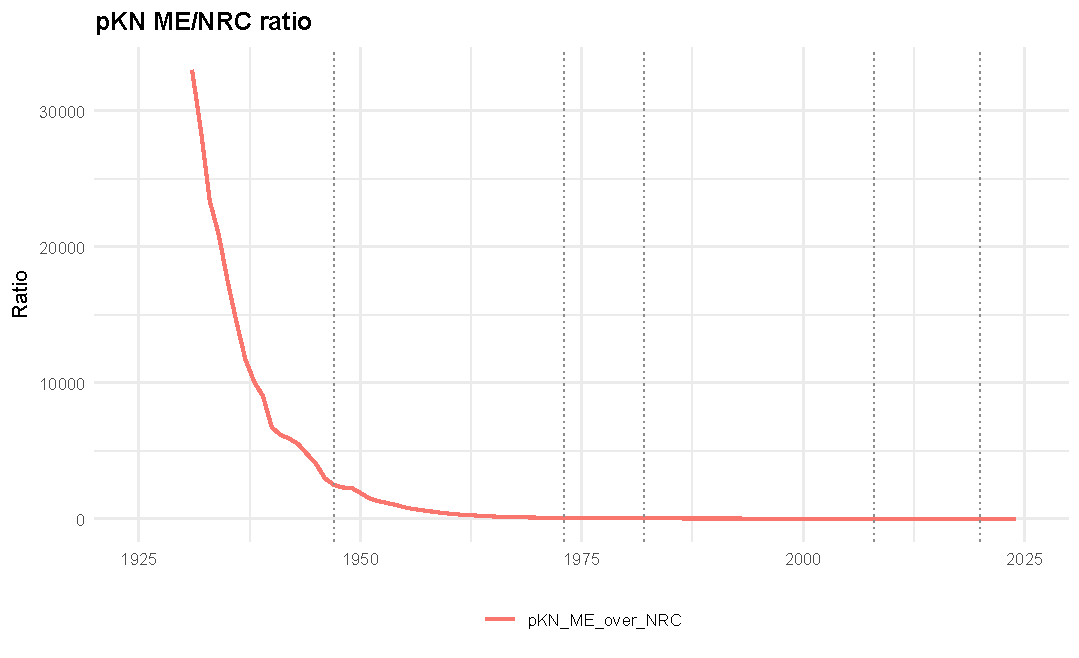
\includegraphics[width=0.92\linewidth]{../figures/D09_fig27_pKN_ME_over_NRC.pdf}
\caption{pKN ME/NRC ratio. D06/D09 pKN and guarded investment-flow diagnostic. The figure helps separate real quantity movements from valuation movements but does not alter pKN or refreeze GPIM stocks.}
\label{fig:D09_fig27_pKN_ME_over_NRC}
\end{figure}

\begin{figure}[H]
\centering
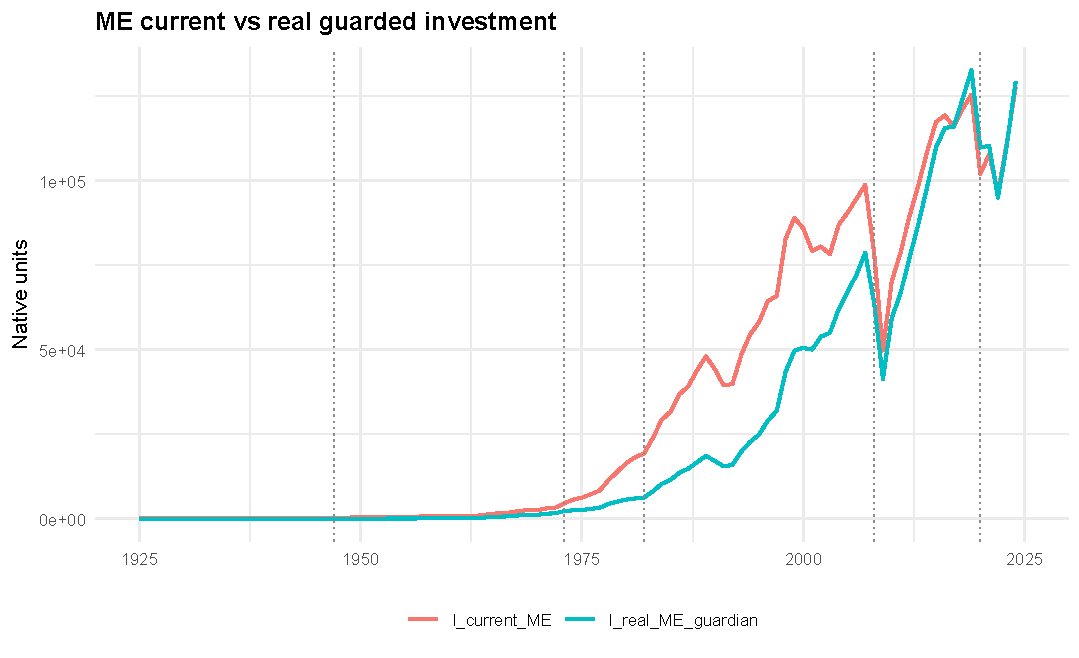
\includegraphics[width=0.92\linewidth]{../figures/D09_fig28_current_vs_real_investment_ME.pdf}
\caption{ME current versus guarded real investment. D06/D09 pKN and guarded investment-flow diagnostic. The figure helps separate real quantity movements from valuation movements but does not alter pKN or refreeze GPIM stocks.}
\label{fig:D09_fig28_current_vs_real_investment_ME}
\end{figure}

\begin{figure}[H]
\centering
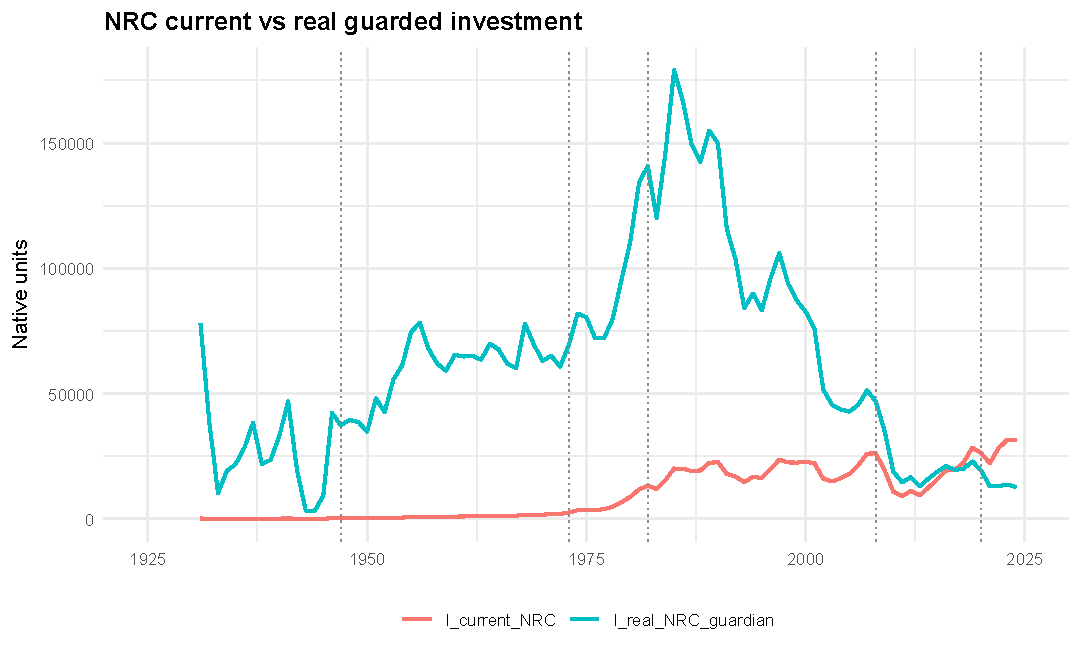
\includegraphics[width=0.92\linewidth]{../figures/D09_fig29_current_vs_real_investment_NRC.pdf}
\caption{NRC current versus guarded real investment. D06/D09 pKN and guarded investment-flow diagnostic. The figure helps separate real quantity movements from valuation movements but does not alter pKN or refreeze GPIM stocks.}
\label{fig:D09_fig29_current_vs_real_investment_NRC}
\end{figure}

\FloatBarrier
\section{Output-Capital Level Relations}
This section restores output-capital figures to the main analytical flow before the human checklist. Figures \textbackslash\{\}ref\{fig:D09\_fig30\_real\_output\_and\_real\_capacity\_levels\}, \textbackslash\{\}ref\{fig:D09\_fig31\_real\_output\_capacity\_ratio\}, \textbackslash\{\}ref\{fig:D09\_fig32\_real\_capacity\_output\_ratio\}, \textbackslash\{\}ref\{fig:D09\_fig33\_nominal\_NFC\_GVA\_and\_current\_capacity\_levels\}, \textbackslash\{\}ref\{fig:D09\_fig34\_nominal\_NFC\_GVA\_current\_capacity\_ratio\}, \textbackslash\{\}ref\{fig:D09\_fig35\_scatter\_Yreal\_NFC\_GVA\_vs\_Kreal\_capacity\}, \textbackslash\{\}ref\{fig:D09\_fig36\_scatter\_Yreal\_NFC\_GVA\_vs\_Kreal\_ME\}, \textbackslash\{\}ref\{fig:D09\_fig37\_scatter\_Yreal\_NFC\_GVA\_vs\_Kreal\_NRC\} show level relations, ratios, and scatterplots for output and capital.

The plots are useful for human plausibility checks: they show whether output and capacity levels move in a way that a later level-analysis design can inspect. There are no fitted lines and no stationarity or cointegration claims.

These figures do not authorize a transformation of μ\_t, K, output, or any ratio for model use.
\begin{figure}[H]
\centering
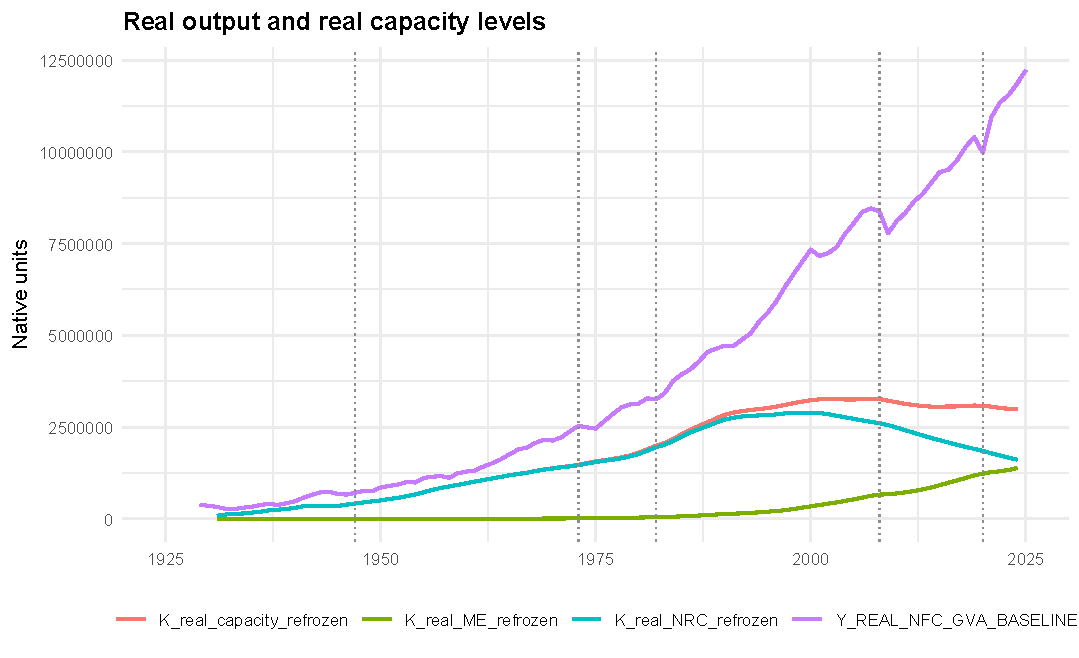
\includegraphics[width=0.92\linewidth]{../figures/D09_fig30_real_output_and_real_capacity_levels.pdf}
\caption{Real output and real capacity levels. D07/D09 level-relation inspection for output and capital. Ratios and scatterplots are REPORT\_ONLY, INSPECTION\_ONLY, and contain no fitted line, coefficient, stationarity test, or transformation authorization.}
\label{fig:D09_fig30_real_output_and_real_capacity_levels}
\end{figure}

\begin{figure}[H]
\centering
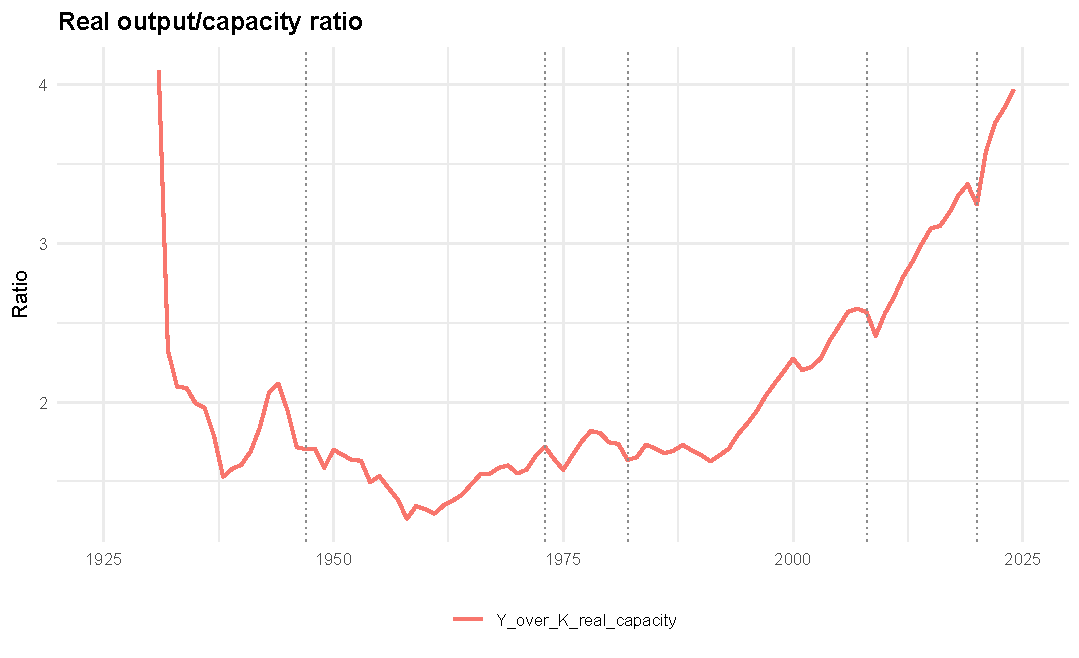
\includegraphics[width=0.92\linewidth]{../figures/D09_fig31_real_output_capacity_ratio.pdf}
\caption{Real output/capacity ratio. D07/D09 level-relation inspection for output and capital. Ratios and scatterplots are REPORT\_ONLY, INSPECTION\_ONLY, and contain no fitted line, coefficient, stationarity test, or transformation authorization.}
\label{fig:D09_fig31_real_output_capacity_ratio}
\end{figure}

\begin{figure}[H]
\centering
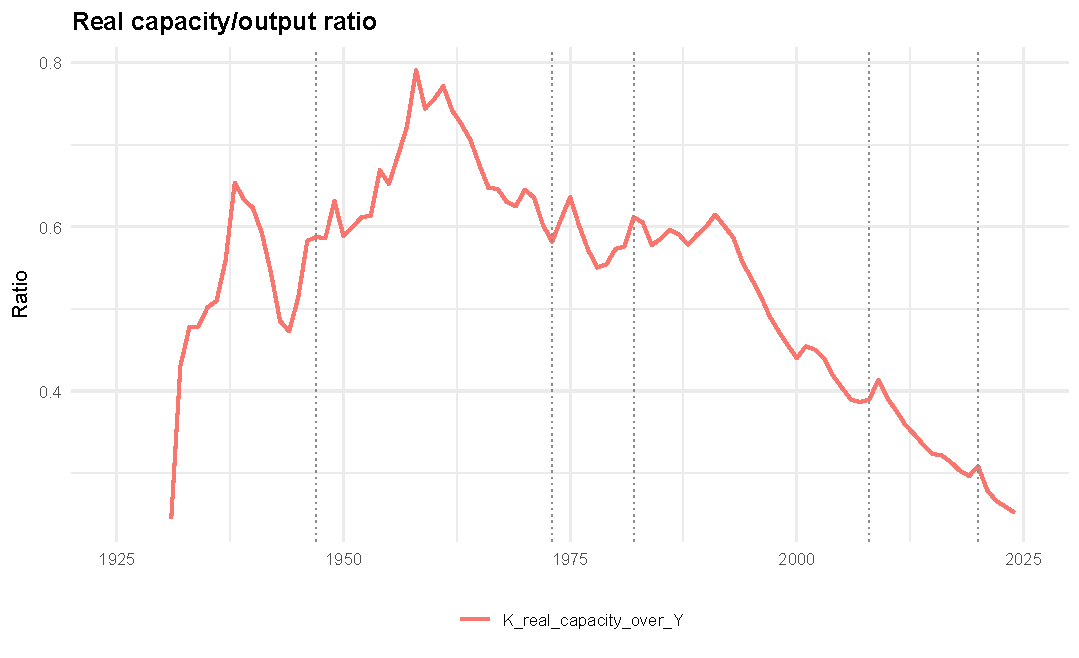
\includegraphics[width=0.92\linewidth]{../figures/D09_fig32_real_capacity_output_ratio.pdf}
\caption{Real capacity/output ratio. D07/D09 level-relation inspection for output and capital. Ratios and scatterplots are REPORT\_ONLY, INSPECTION\_ONLY, and contain no fitted line, coefficient, stationarity test, or transformation authorization.}
\label{fig:D09_fig32_real_capacity_output_ratio}
\end{figure}

\begin{figure}[H]
\centering
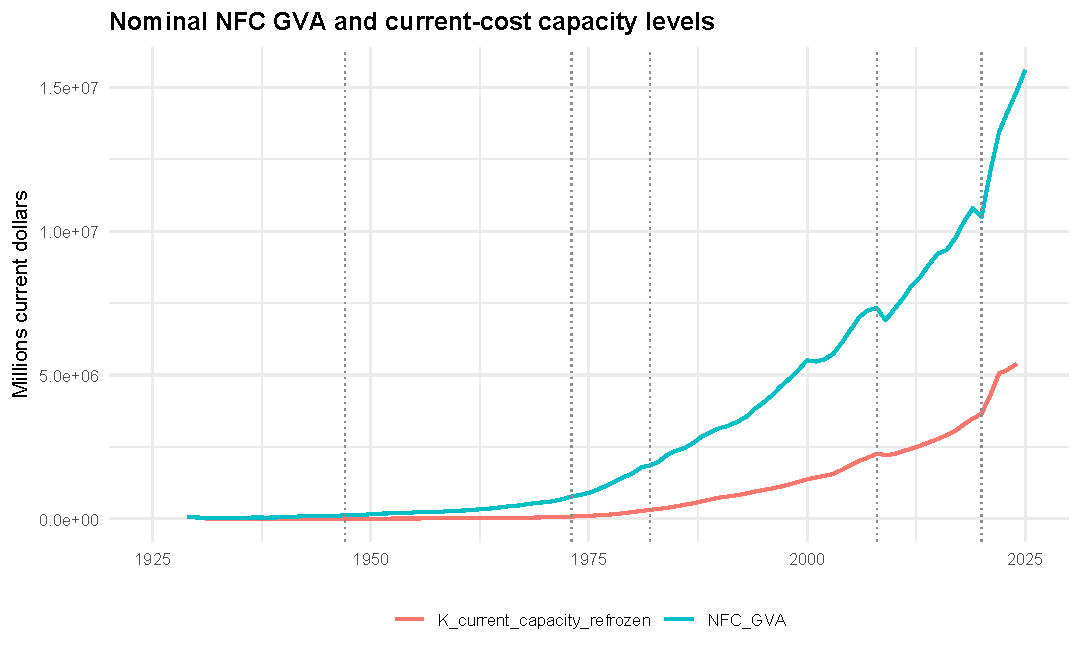
\includegraphics[width=0.92\linewidth]{../figures/D09_fig33_nominal_NFC_GVA_and_current_capacity_levels.pdf}
\caption{Nominal NFC GVA and current-cost capacity levels. D07/D09 level-relation inspection for output and capital. Ratios and scatterplots are REPORT\_ONLY, INSPECTION\_ONLY, and contain no fitted line, coefficient, stationarity test, or transformation authorization.}
\label{fig:D09_fig33_nominal_NFC_GVA_and_current_capacity_levels}
\end{figure}

\begin{figure}[H]
\centering
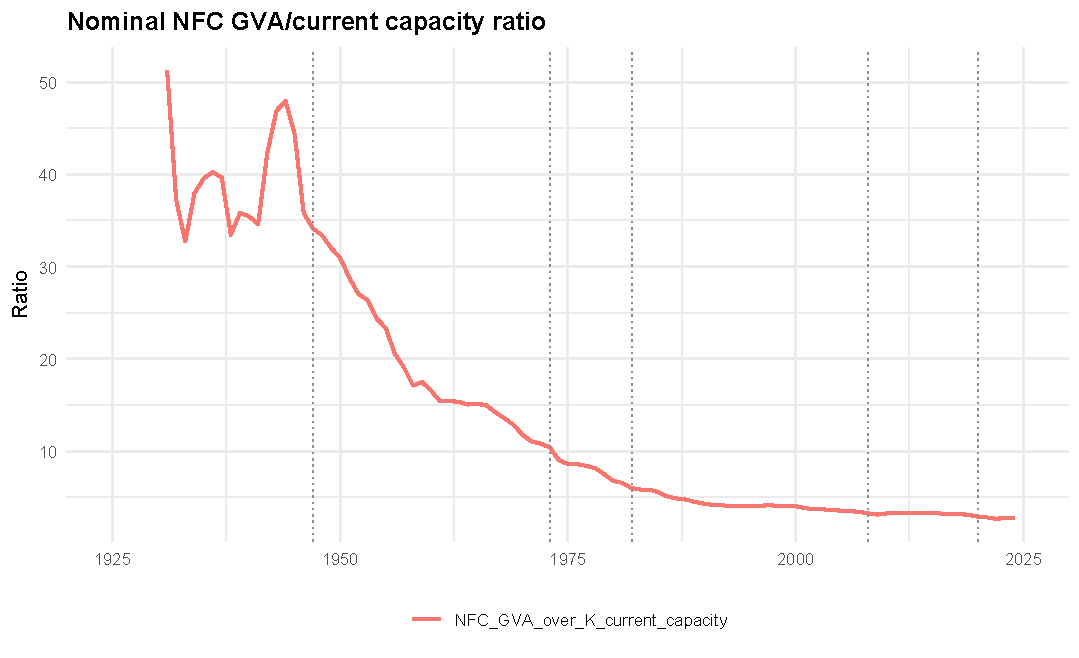
\includegraphics[width=0.92\linewidth]{../figures/D09_fig34_nominal_NFC_GVA_current_capacity_ratio.pdf}
\caption{Nominal NFC GVA/current-capacity ratio. D07/D09 level-relation inspection for output and capital. Ratios and scatterplots are REPORT\_ONLY, INSPECTION\_ONLY, and contain no fitted line, coefficient, stationarity test, or transformation authorization.}
\label{fig:D09_fig34_nominal_NFC_GVA_current_capacity_ratio}
\end{figure}

\begin{figure}[H]
\centering
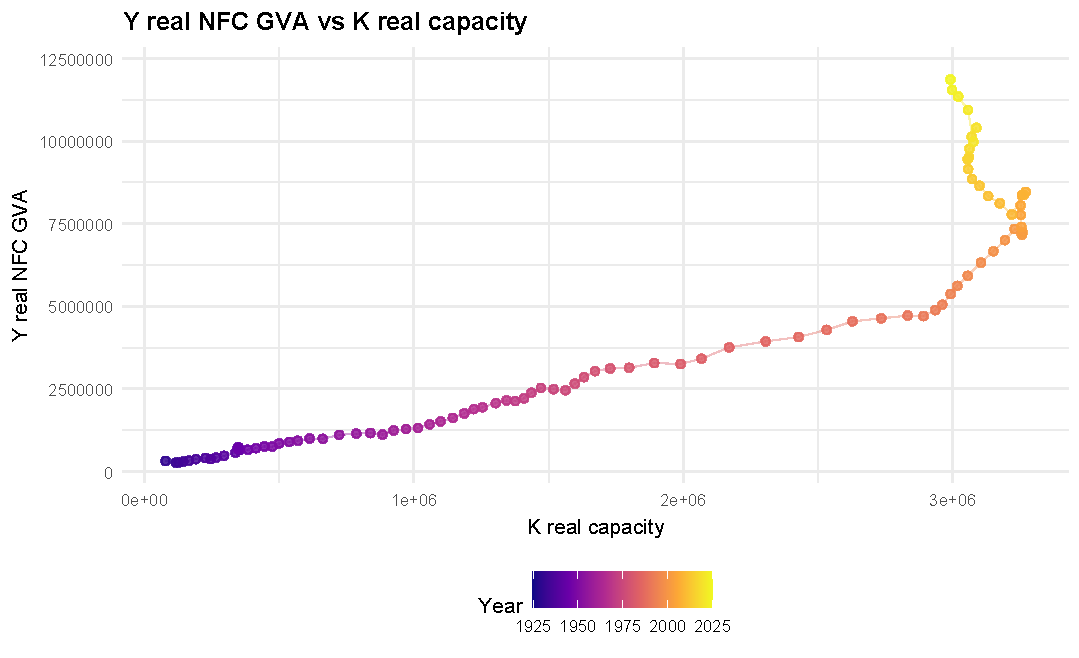
\includegraphics[width=0.92\linewidth]{../figures/D09_fig35_scatter_Yreal_NFC_GVA_vs_Kreal_capacity.pdf}
\caption{Y real NFC GVA versus K real capacity. D07/D09 level-relation inspection for output and capital. Ratios and scatterplots are REPORT\_ONLY, INSPECTION\_ONLY, and contain no fitted line, coefficient, stationarity test, or transformation authorization.}
\label{fig:D09_fig35_scatter_Yreal_NFC_GVA_vs_Kreal_capacity}
\end{figure}

\begin{figure}[H]
\centering
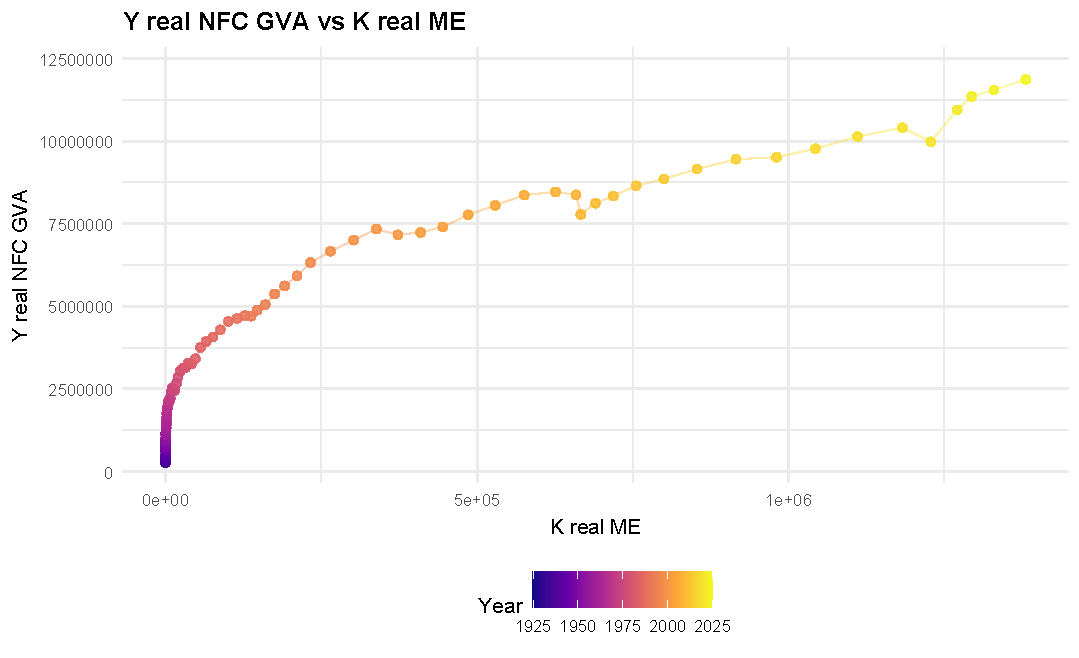
\includegraphics[width=0.92\linewidth]{../figures/D09_fig36_scatter_Yreal_NFC_GVA_vs_Kreal_ME.pdf}
\caption{Y real NFC GVA versus K real ME. D07/D09 level-relation inspection for output and capital. Ratios and scatterplots are REPORT\_ONLY, INSPECTION\_ONLY, and contain no fitted line, coefficient, stationarity test, or transformation authorization.}
\label{fig:D09_fig36_scatter_Yreal_NFC_GVA_vs_Kreal_ME}
\end{figure}

\begin{figure}[H]
\centering
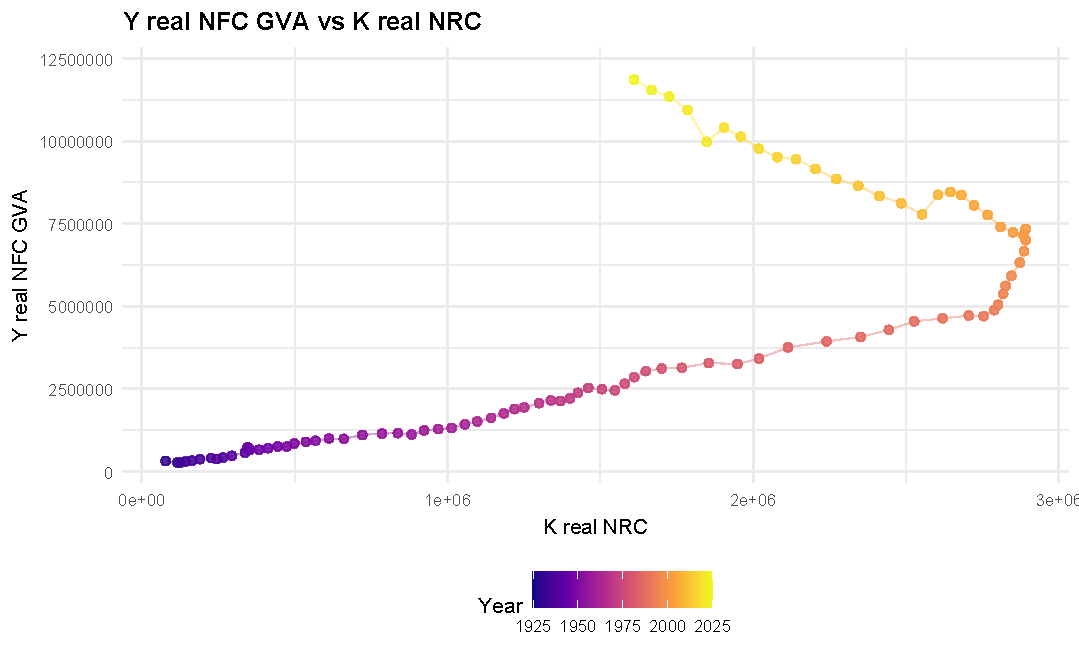
\includegraphics[width=0.92\linewidth]{../figures/D09_fig37_scatter_Yreal_NFC_GVA_vs_Kreal_NRC.pdf}
\caption{Y real NFC GVA versus K real NRC. D07/D09 level-relation inspection for output and capital. Ratios and scatterplots are REPORT\_ONLY, INSPECTION\_ONLY, and contain no fitted line, coefficient, stationarity test, or transformation authorization.}
\label{fig:D09_fig37_scatter_Yreal_NFC_GVA_vs_Kreal_NRC}
\end{figure}

\FloatBarrier
\section{Distribution and Surplus-Share Inspection}
This section keeps all distribution figures in the distribution section rather than orphaning them in an appendix. Figures \textbackslash\{\}ref\{fig:D09\_fig38\_NFC\_wage\_share\_variants\}, \textbackslash\{\}ref\{fig:D09\_fig39\_NFC\_gross\_net\_surplus\_share\_variants\}, \textbackslash\{\}ref\{fig:D09\_fig40\_NFC\_CFC\_share\}, \textbackslash\{\}ref\{fig:D09\_fig41\_CORP\_wage\_share\_reconciliation\_variants\}, \textbackslash\{\}ref\{fig:D09\_fig42\_CORP\_surplus\_share\_reconciliation\_variants\} show wage, surplus, CFC, and corporate reconciliation variants.

The figures preserve the D07 status distinctions between baseline shares, reconciliation variants, and report-only scaffolds. This keeps surplus-share inspection inside the accounting boundary.

No distribution series is promoted beyond its D07 authorization status, and no transformation use is authorized.
\begin{figure}[H]
\centering
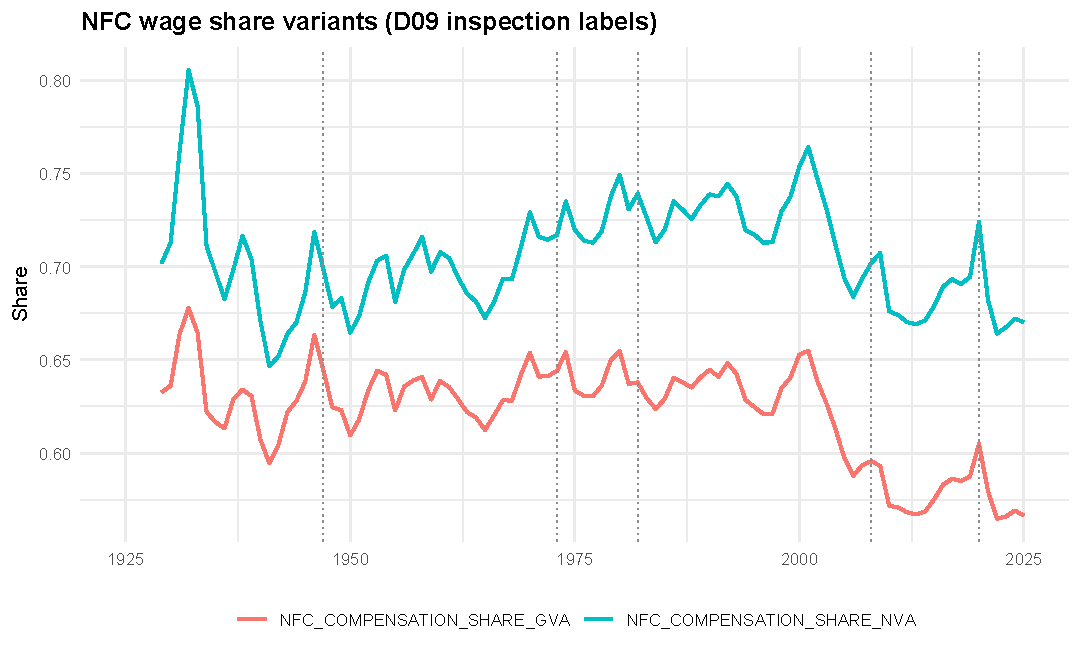
\includegraphics[width=0.92\linewidth]{../figures/D09_fig38_NFC_wage_share_variants.pdf}
\caption{NFC wage share variants. D07/D09 distribution inspection figure. Authorized baseline shares remain distinguished from reconciliation and report-only scaffolds; no distribution variable is promoted beyond its D07 status.}
\label{fig:D09_fig38_NFC_wage_share_variants}
\end{figure}

\begin{figure}[H]
\centering
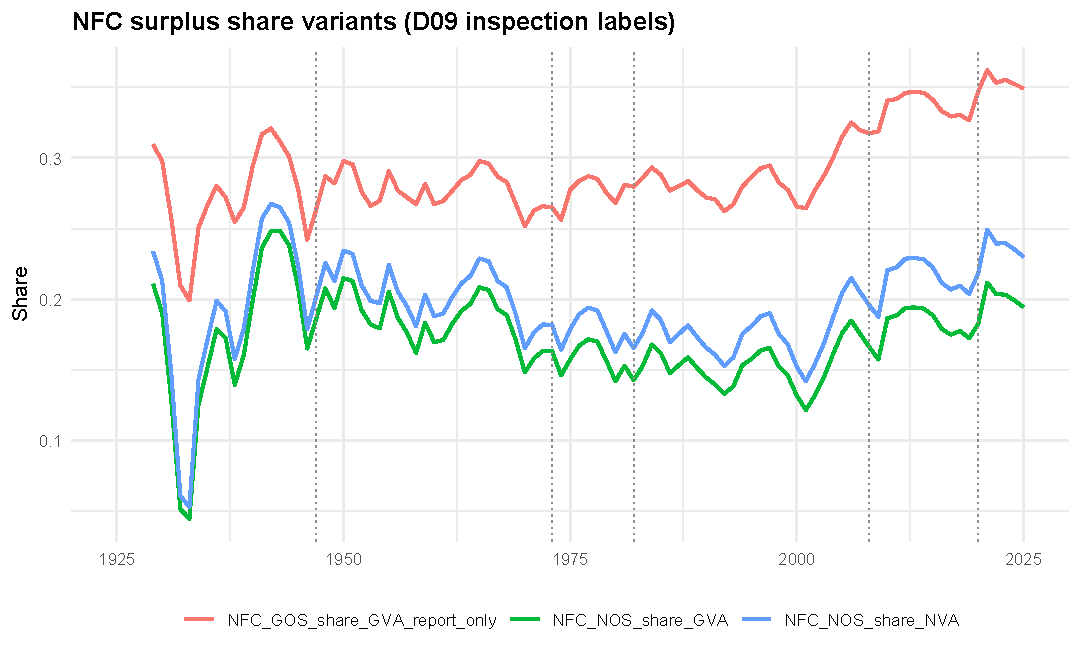
\includegraphics[width=0.92\linewidth]{../figures/D09_fig39_NFC_gross_net_surplus_share_variants.pdf}
\caption{NFC surplus share variants. D07/D09 distribution inspection figure. Authorized baseline shares remain distinguished from reconciliation and report-only scaffolds; no distribution variable is promoted beyond its D07 status.}
\label{fig:D09_fig39_NFC_gross_net_surplus_share_variants}
\end{figure}

\begin{figure}[H]
\centering
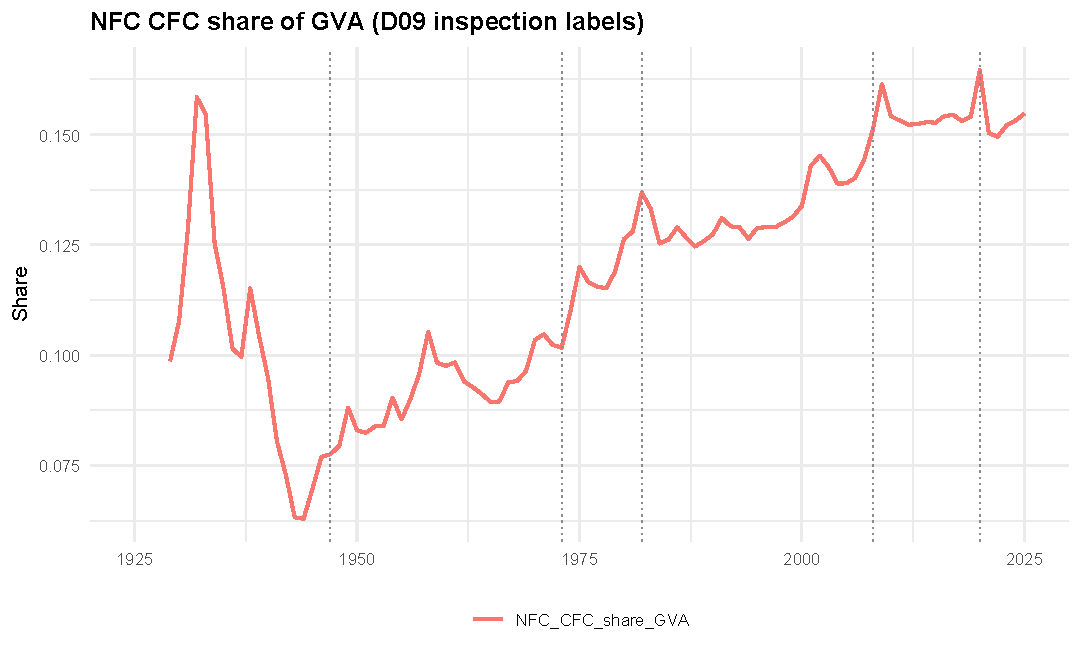
\includegraphics[width=0.92\linewidth]{../figures/D09_fig40_NFC_CFC_share.pdf}
\caption{NFC CFC share. D07/D09 distribution inspection figure. Authorized baseline shares remain distinguished from reconciliation and report-only scaffolds; no distribution variable is promoted beyond its D07 status.}
\label{fig:D09_fig40_NFC_CFC_share}
\end{figure}

\begin{figure}[H]
\centering
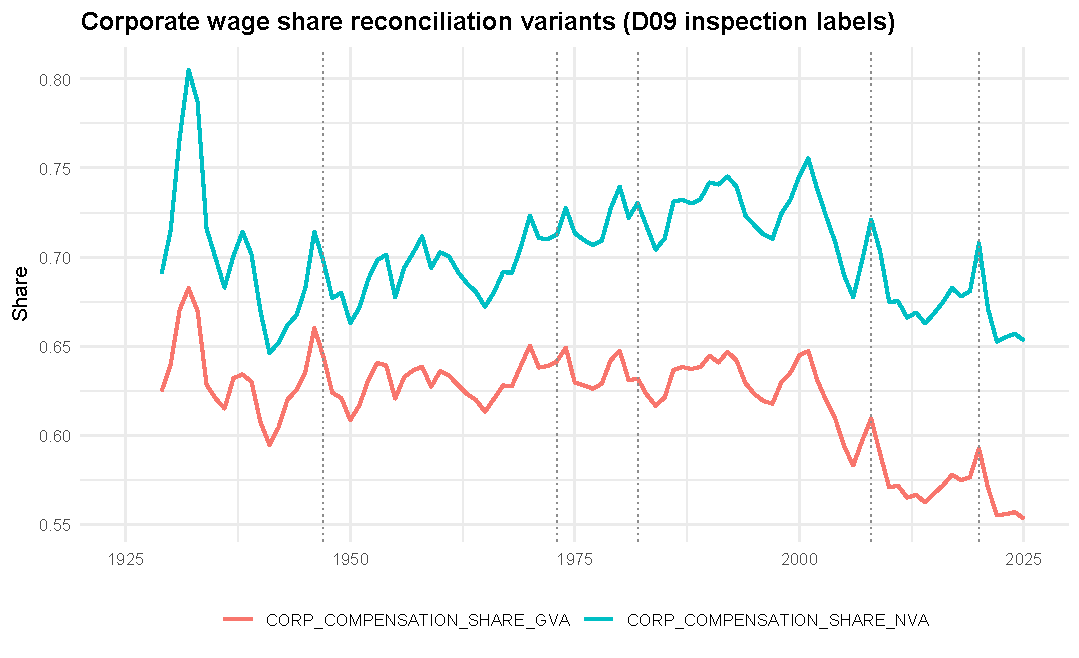
\includegraphics[width=0.92\linewidth]{../figures/D09_fig41_CORP_wage_share_reconciliation_variants.pdf}
\caption{Corporate wage share reconciliation variants. D07/D09 distribution inspection figure. Authorized baseline shares remain distinguished from reconciliation and report-only scaffolds; no distribution variable is promoted beyond its D07 status.}
\label{fig:D09_fig41_CORP_wage_share_reconciliation_variants}
\end{figure}

\begin{figure}[H]
\centering
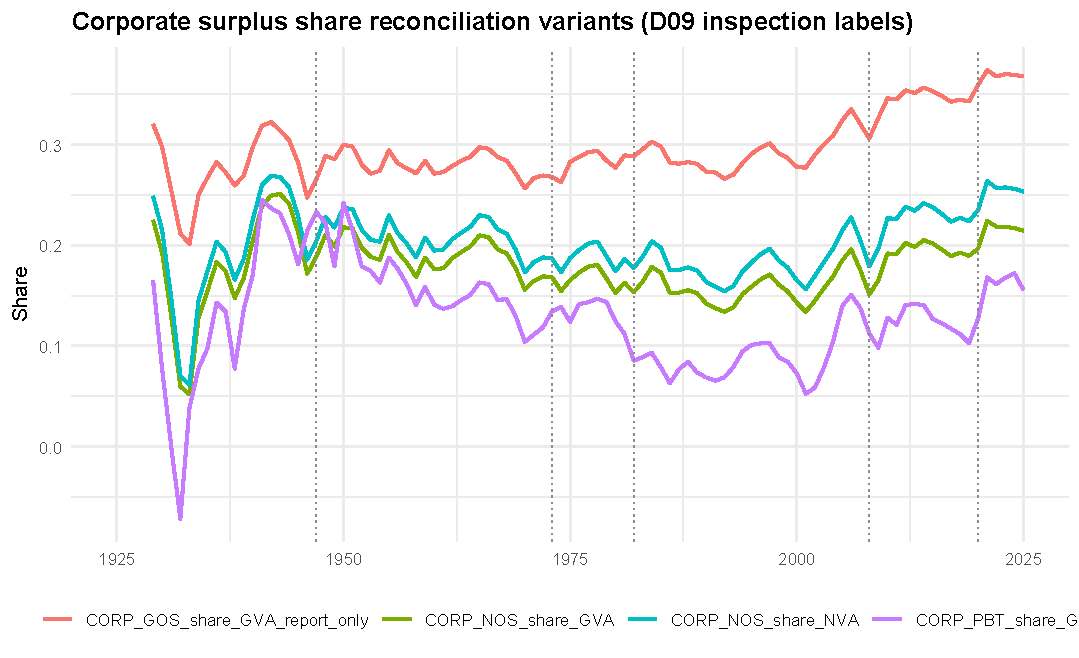
\includegraphics[width=0.92\linewidth]{../figures/D09_fig42_CORP_surplus_share_reconciliation_variants.pdf}
\caption{Corporate surplus share reconciliation variants. D07/D09 distribution inspection figure. Authorized baseline shares remain distinguished from reconciliation and report-only scaffolds; no distribution variable is promoted beyond its D07 status.}
\label{fig:D09_fig42_CORP_surplus_share_reconciliation_variants}
\end{figure}

\FloatBarrier
\section{Financial-Sector Transfer and Double-Counting Safeguards}
This section places the financial-transfer safeguard where it is interpreted. Figure \textbackslash\{\}ref\{fig:D09\_fig43\_surplus\_accounting\_ladder\_bridge\} is read after the table-first safeguard statement.

The financial ladder is a boundary device: productive-origin surplus, accounting reconciliation, financial-transfer layers, and imputed-interest corrections must not be silently collapsed into one profit object.

The section does not authorize financial correction as baseline productive-origin surplus.
\input{../tables/D09_R_table_financial_transfer_double_counting_safeguard.tex}
\begin{figure}[H]
\centering
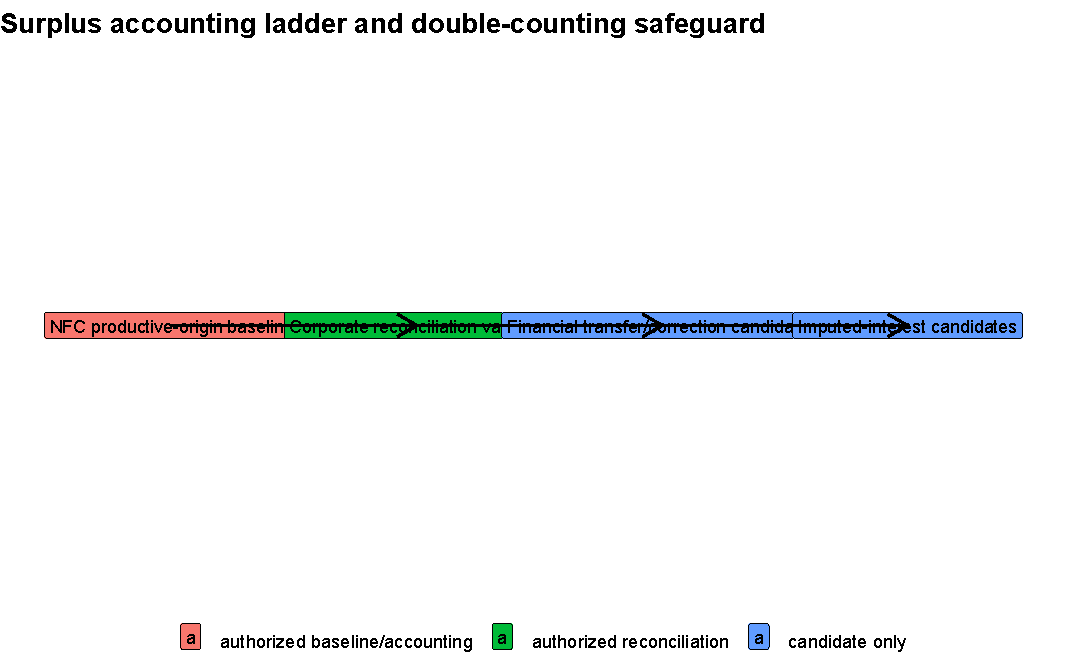
\includegraphics[width=0.92\linewidth]{../figures/D09_fig43_surplus_accounting_ladder_bridge.pdf}
\caption{Surplus accounting ladder and double-counting safeguard. Financial-transfer safeguard diagnostic from D09. The table-first interpretation separates productive-origin surplus from financial correction and imputed-interest layers, preventing double counting or boundary leakage.}
\label{fig:D09_fig43_surplus_accounting_ladder_bridge}
\end{figure}

\FloatBarrier
\section{Capital-Output-Distribution Relational Inspection}
This section collects the relational scatterplots after their ingredients have been shown. Figures \textbackslash\{\}ref\{fig:D09\_fig44\_wage\_share\_vs\_ME\_over\_NRC\}, \textbackslash\{\}ref\{fig:D09\_fig45\_wage\_share\_vs\_ME\_share\_of\_capacity\}, \textbackslash\{\}ref\{fig:D09\_fig46\_wage\_share\_vs\_capacity\_output\_ratio\}, \textbackslash\{\}ref\{fig:D09\_fig47\_surplus\_share\_vs\_ME\_over\_NRC\}, \textbackslash\{\}ref\{fig:D09\_fig48\_surplus\_share\_vs\_capacity\_output\_ratio\} relate distribution shares to ME/NRC and capacity-output diagnostics.

These plots are visual inspection only. The absence of fitted lines is intentional: D09-R is not estimating a relation or testing a model.

No coefficient, fitted relation, or transformation is authorized here.
\begin{figure}[H]
\centering
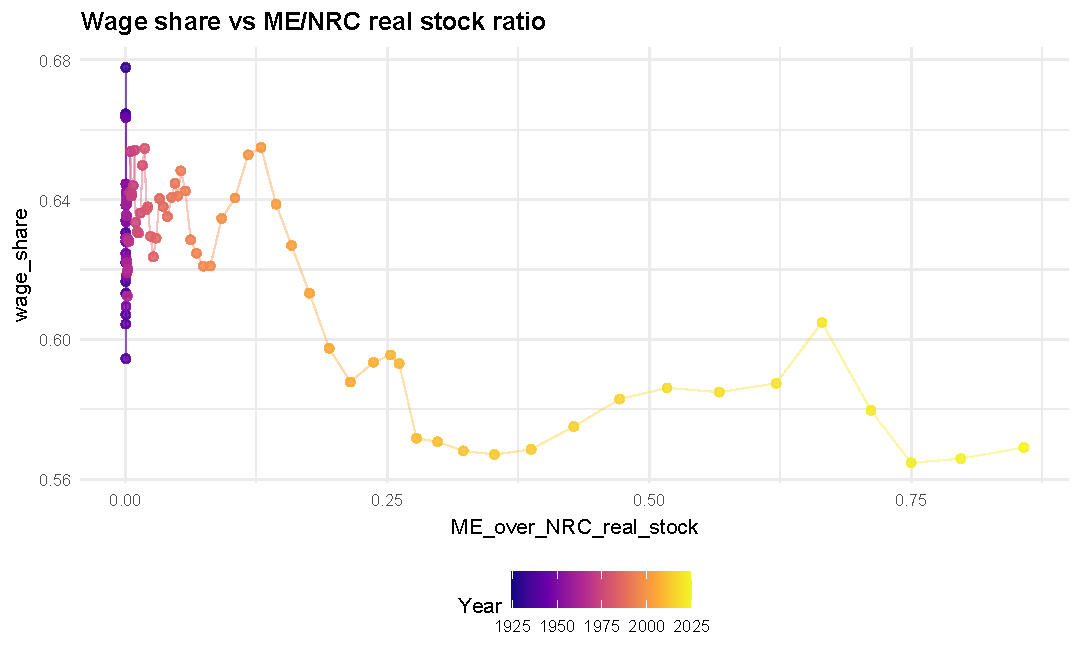
\includegraphics[width=0.92\linewidth]{../figures/D09_fig44_wage_share_vs_ME_over_NRC.pdf}
\caption{Wage share versus ME/NRC real stock ratio. D09 report-only relational inspection. The figure is visual only, uses no fitted line, and does not authorize transformation or econometric use.}
\label{fig:D09_fig44_wage_share_vs_ME_over_NRC}
\end{figure}

\begin{figure}[H]
\centering
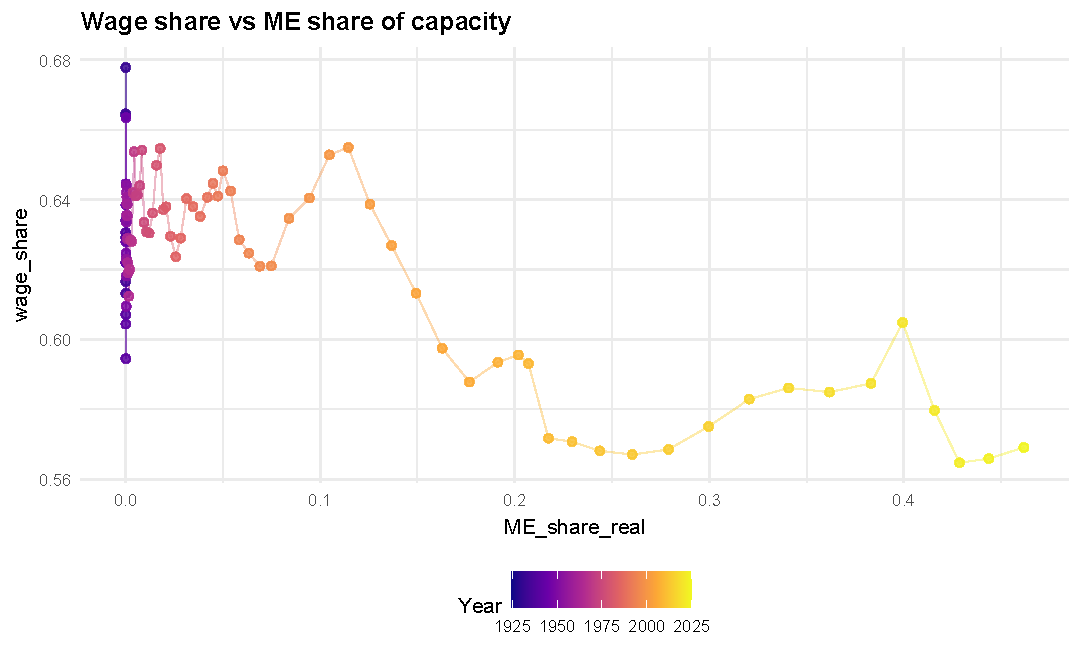
\includegraphics[width=0.92\linewidth]{../figures/D09_fig45_wage_share_vs_ME_share_of_capacity.pdf}
\caption{Wage share versus ME share of capacity. D09 report-only relational inspection. The figure is visual only, uses no fitted line, and does not authorize transformation or econometric use.}
\label{fig:D09_fig45_wage_share_vs_ME_share_of_capacity}
\end{figure}

\begin{figure}[H]
\centering
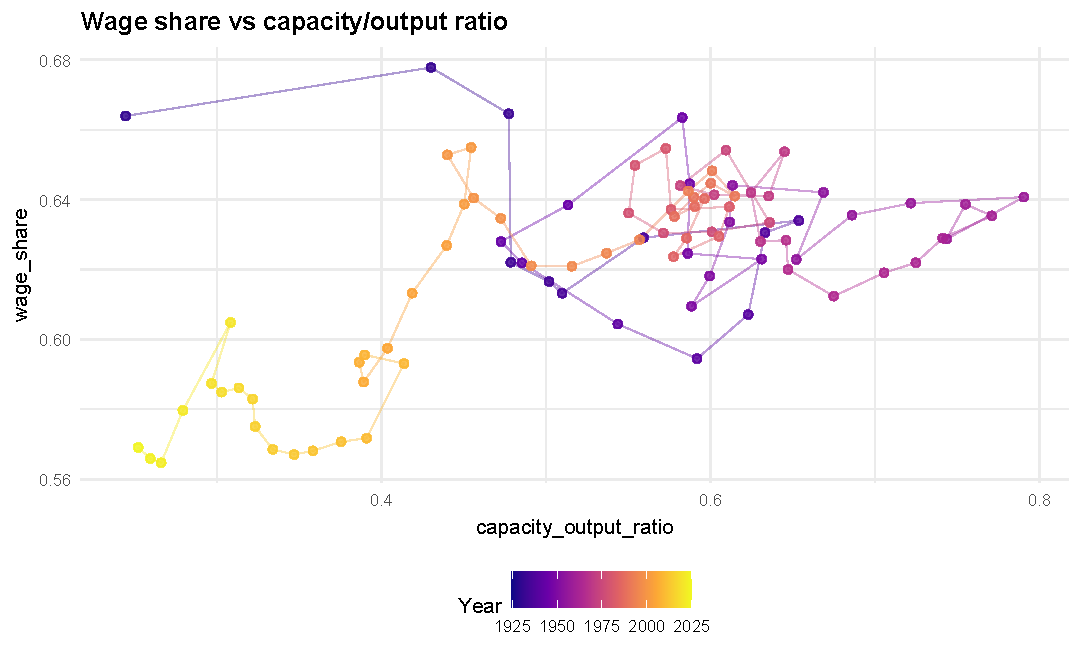
\includegraphics[width=0.92\linewidth]{../figures/D09_fig46_wage_share_vs_capacity_output_ratio.pdf}
\caption{Wage share versus capacity/output ratio. D09 report-only relational inspection. The figure is visual only, uses no fitted line, and does not authorize transformation or econometric use.}
\label{fig:D09_fig46_wage_share_vs_capacity_output_ratio}
\end{figure}

\begin{figure}[H]
\centering
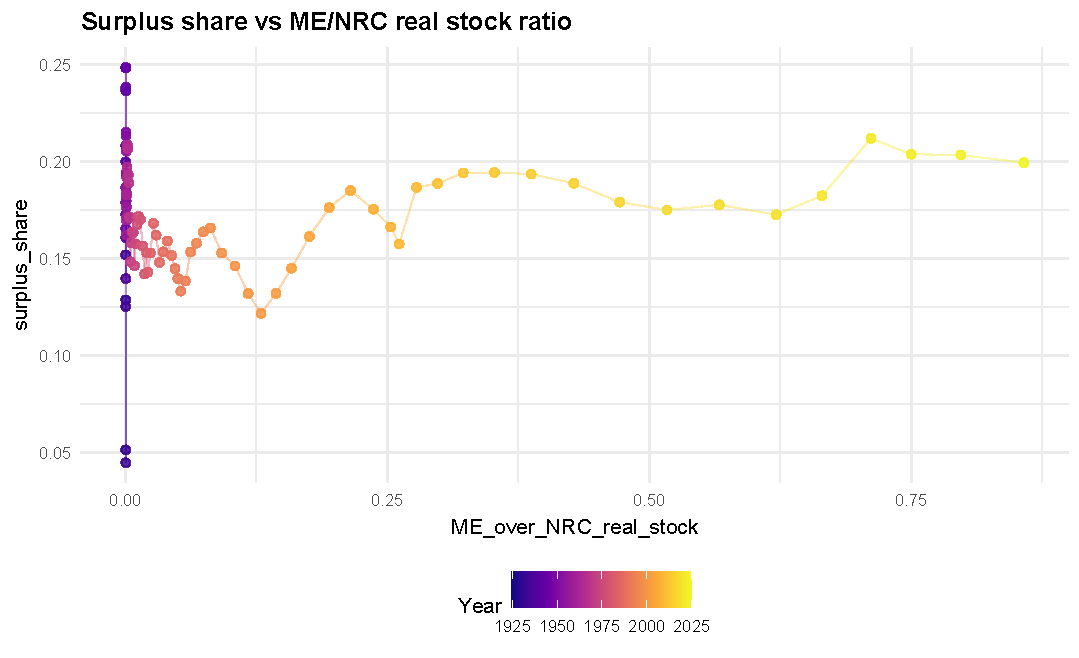
\includegraphics[width=0.92\linewidth]{../figures/D09_fig47_surplus_share_vs_ME_over_NRC.pdf}
\caption{Surplus share versus ME/NRC real stock ratio. D09 report-only relational inspection. The figure is visual only, uses no fitted line, and does not authorize transformation or econometric use.}
\label{fig:D09_fig47_surplus_share_vs_ME_over_NRC}
\end{figure}

\begin{figure}[H]
\centering
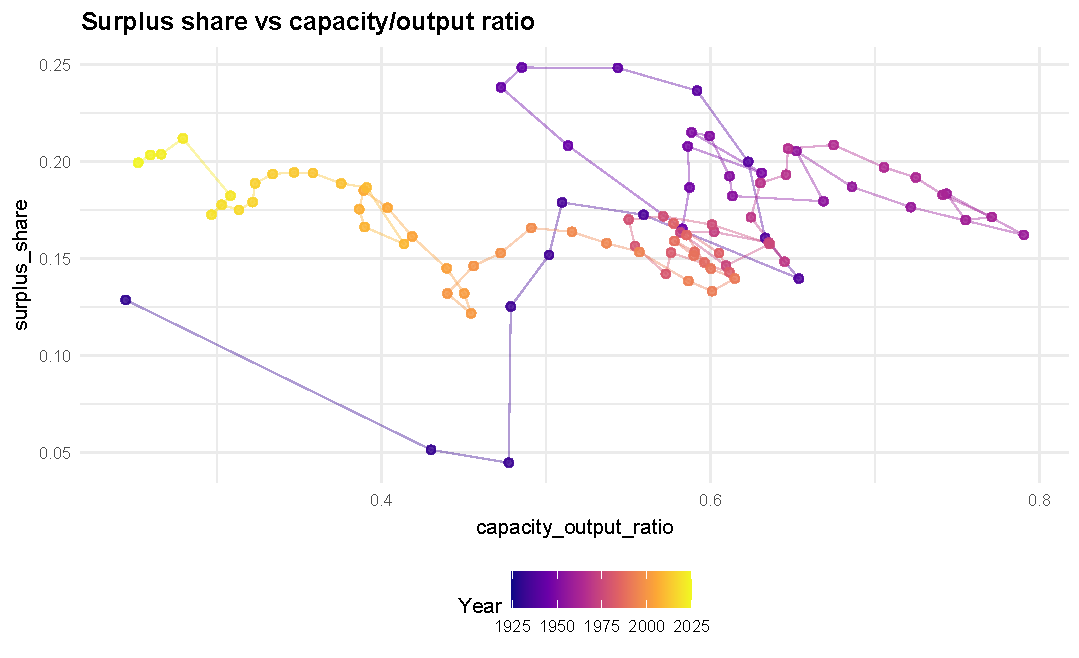
\includegraphics[width=0.92\linewidth]{../figures/D09_fig48_surplus_share_vs_capacity_output_ratio.pdf}
\caption{Surplus share versus capacity/output ratio. D09 report-only relational inspection. The figure is visual only, uses no fitted line, and does not authorize transformation or econometric use.}
\label{fig:D09_fig48_surplus_share_vs_capacity_output_ratio}
\end{figure}

\FloatBarrier
\section{Human Interpretation of the NRC Decline}
The NRC decline can be defended only with the correct object definition. The object is nonfinancial productive-capacity nonresidential construction, not total nonresidential buildings and not all standing structures.

The defensible interpretation is boundary movement: abandonment, rezoning, conversion to residential use, or absorption into financial/real-estate uses can remove structures from the productive-capacity object without literal demolition. That interpretation is plausible, but the L=30 service-life assumption and short NRC warmup leave a medium review-required risk.

This section does not resolve the service-life issue. It makes the issue explicit and prevents the report from overstating the physical meaning of the real NRC stock.
\FloatBarrier
\section{Future Sensitivity Design: NRC Service Life and Warmup}
This section records a future sensitivity design without executing it. The proposed pass would compare longer NRC service lives and possibly a longer infrastructure-style survival profile if literature supports it.

The future design keeps the baseline intact: NRC L=30, alpha=1.6 remains the D06/D07/D09 object. Alternatives such as L=40, L=50, and L=60 are proposed future report-only cases, not D09-R results.

D09-R does not run sensitivity analysis and does not authorize D10 transformation planning.

\begin{tabular}{lllllll}
\toprule
reference\_key & author\_year & asset\_scope & reported\_service\_life\_or\_depreciation\_basis & relevance\_to\_NRC & source\_status & notes\\
\midrule
Nomura2005\_NRC\_service\_life\_REVIEW & Nomura 2005 & nonresidential structures / infrastructure / capital measurement & SOURCE\_REQUIRED & Potential external check on NRC service-life plausibility. & SOURCE\_REQUIRED & Do not assert service-life values until the source is retrieved and verified.\\
BEA\_fixed\_assets\_service\_life\_documentation\_REVIEW & BEA fixed assets documentation & fixed assets and depreciation/service-life assumptions & SOURCE\_REQUIRED & Potential source for U.S. fixed-asset service-life conventions. & SOURCE\_REQUIRED & Do not assert service-life values until official documentation is retrieved and verified.\\
OECD\_capital\_measurement\_manual\_REVIEW & OECD capital measurement manual & capital measurement, PIM, service lives, depreciation & SOURCE\_REQUIRED & Potential capital-measurement framing for service-life sensitivity. & SOURCE\_REQUIRED & Do not assert service-life values until the manual is retrieved and verified.\\
Hulten\_Wykoff\_depreciation\_literature\_REVIEW & Hulten-Wykoff depreciation literature & depreciation and asset lives & SOURCE\_REQUIRED & Potential depreciation/service-life background. & SOURCE\_REQUIRED & Do not assert service-life values until the literature is retrieved and verified.\\
local\_repo\_GPIM\_service\_life\_context\_REVIEW & Local repo context & D01-D06 GPIM service-life implementation notes & Local code records the locked D06 baseline L=30, alpha=1.6; not external validation. & Confirms the local baseline and no-terminal-cliff rule, but does not settle external plausibility. & LOCAL\_CONTEXT\_ONLY & Local source candidates: codes/US\_D06\_gpim\_refreeze\_with\_guarded\_pkn.R; reports/report\_gpim\_shaikh\_comparison\_2026-06-25/report\_gpim\_shaikh\_comparison\_2026-06-25.md\\
\bottomrule
\end{tabular}

\FloatBarrier
\section{Human Decision Checklist}
The checklist records the human-facing outcome after layout repair and NRC interpretation repair.

The report is ready for D09 double validation review with the NRC service-life issue carried as medium review-required.

The checklist does not authorize model transformations or D10 implementation.

\begin{tabular}{lllll}
\toprule
item & status & evidence & recommended\_decision & notes\\
\midrule
Revised report figure placement is aligned with section text & PASS & D09\_R\_figure\_placement\_ledger.csv and revised PDF & accept & D09-R repairs report layout and interpretation only; it does not start D10 transformation planning.\\
NRC decline interpretation is explicit and boundary-safe & PASS & Sections 4, 6, 16, and NRC service-life interpretation ledger & accept & D09-R repairs report layout and interpretation only; it does not start D10 transformation planning.\\
NRC L=30 and warmup concern are carried forward & REVIEW\_REQUIRED & D08/D09 NRC warmup flag retained as medium review-required & carry forward & D09-R repairs report layout and interpretation only; it does not start D10 transformation planning.\\
No GPIM rebuild, survival change, pKN change, or econometrics are run & PASS & D09-R script copies prior D09 figures and writes report-only ledgers & accept & D09-R repairs report layout and interpretation only; it does not start D10 transformation planning.\\
Future sensitivity is proposed but not executed & PASS & D09\_R\_future\_NRC\_service\_life\_sensitivity\_design.md & accept & D09-R repairs report layout and interpretation only; it does not start D10 transformation planning.\\
\addlinespace
Ready for D09 double validation review & PASS\_WITH\_REVIEW\_FLAG & All validation checks pass with one non-blocking NRC review flag & AUTHORIZE\_D09\_DOUBLE\_VALIDATION\_REVIEW & D09-R repairs report layout and interpretation only; it does not start D10 transformation planning.\\
\bottomrule
\end{tabular}

\FloatBarrier
\appendix
\section{Secondary Figures}
No D09 figure is orphaned in the appendix in this repaired report. The parked/excluded status view appears in Section 10 because it is needed to explain boundary status, not because it is a baseline alternative.
\section{Audit Tables}
The revised validation checks, human review flags, NRC interpretation ledger, and service-life literature placeholders are written to the D09-R csv and tables folders. Large ledgers remain CSV-first to avoid overfull main-body tables.
\section{Figure Manifest}
The revised figure-placement ledger records one placement decision for each of the 48 copied D09 figures. The source figure manifest remains D09\_figure\_manifest.csv; the repaired placement ledger is D09\_R\_figure\_placement\_ledger.csv.
\end{document}
